\documentclass[11pt, a4paper]{article}

%---------------------------------------------------------
% Lingua E Codifica
%---------------------------------------------------------
\usepackage[italian]{babel}
\usepackage[T1]{fontenc}
\usepackage{lmodern}

%---------------------------------------------------------
% Layout Di Pagina E Tipografia
%---------------------------------------------------------
\usepackage[margin=2cm, top=1.5cm, bottom=1.5cm]{geometry}
\usepackage{parskip}
\usepackage[expansion=false]{microtype}

%---------------------------------------------------------
% Gestione Dei Colori
%---------------------------------------------------------
\usepackage[table]{xcolor}

%---------------------------------------------------------
% Matematica E Simboli
%---------------------------------------------------------
\usepackage{amsmath, amssymb, amsfonts}
\usepackage{mathtools}
\usepackage{siunitx}

% BB OTTIMIZZAZIONE MATRICI LUNGHE PER LA STAMPA
\setlength{\arraycolsep}{10pt}
\usepackage{bm}
\usepackage{arydshln}

%---------------------------------------------------------
% Grafica, Immagini E Tabelle
%---------------------------------------------------------
\usepackage{graphicx}
\graphicspath{{./Images/Appunti}}
\usepackage{float}
\usepackage{booktabs}
\usepackage{array}
\usepackage{multirow}
\usepackage{tabularx}
\usepackage{listings}
\usepackage{tikz}
\usetikzlibrary{shapes.geometric, arrows.meta, positioning, calc, quotes}

%---------------------------------------------------------
% Link, Riferimenti Ed Elenchi
%---------------------------------------------------------
\usepackage[unicode]{hyperref}
\hypersetup{
    colorlinks=true,
    linkcolor=blue,
    urlcolor=blue,
    citecolor=blue,
    pdftitle={Capitolo 3},
    pdfauthor={Francesco Lo Verde},
    pdfpagemode=FullScreen,
}
\usepackage{bookmark}
\usepackage[italian,capitalize]{cleveref}
\usepackage{enumitem}
\setlist{noitemsep}

%---------------------------------------------------------
% Personalizzazione Titoli E Altri Pacchetti
%---------------------------------------------------------
\usepackage{titlesec}
\titleformat{\section}{\normalfont\LARGE\bfseries}{\thesection}{1em}{}
\titleformat{\subsection}{\normalfont\Large\bfseries}{\thesubsection}{1em}{}
\titleformat{\subsubsection}{\normalfont\large\bfseries}{\thesubsubsection}{1em}{}

\usepackage{comment}
\newtheorem{theorem}{Definizione}
\newcommand{\commento}[1]{\textcolor{blue}{\textit{#1}}}

\author{Francesco Lo Verde}
\begin{document}

\section{Cinematica Differenziale}
La cinematica differenziale stabilisce una relazione fondamentale tra le velocità nello spazio dei giunti e le velocità dell'end-effector nello spazio operativo. L'obiettivo è mappare la velocità dei giunti, descritta dal vettore \(\dot{\bm{q}}\), alla velocità lineare e angolare dell'end effector.

Un corpo viene definito \textbf{rigido} se la distanza euclidea tra due qualsiasi suoi punti rimane invariata nel tempo, indipendentemente dal moto del corpo stesso. Consideriamo due punti \(\bm{p}_1\) e \(\bm{p}_2\) appartenenti a tale corpo. Il vettore che congiunge questi due punti è dato da:
\[
    \bm{r}_{12}(t) = \bm{p}_1(t) - \bm{p}_2(t)
\]
Sebbene la traslazione e la rotazione del corpo modifichino l'orientamento del vettore \(\bm{r}_{12}(t)\) nello spazio, la sua norma, che rappresenta la distanza tra i punti, deve rimanere costante.\\
Per tradurre questa condizione geometrica in una relazione tra le velocità, è più conveniente operare sul quadrato della norma, la cui costanza è equivalente. La sua derivata totale rispetto al tempo deve essere, di conseguenza, nulla. Utilizzando la notazione vettoriale, il quadrato della norma è \(\bm{r}_{12}^T(t) \bm{r}_{12}(t)\). Si ha quindi:
\[
    \frac{d}{dt} \left( \frac{1}{2} \| \bm{r}_{12}(t) \|^2 \right) = \frac{d}{dt} \left( \frac{1}{2} \bm{r}_{12}^T(t) \bm{r}_{12}(t) \right) = 0
\]
Applicando la regola di derivazione del prodotto, si ottiene:
\[
    \frac{1}{2} \biggl[ \dot{\bm{r}}_{12}^T(t) \bm{r}_{12}(t) + \bm{r}_{12}^T(t) \dot{\bm{r}}_{12}(t) \biggr] = 0
\]
I due termini dentro la parentesi sono uguali quindi:
\[
    \frac{1}{2} \biggl[ 2 \; \dot{\bm{r}}_{12}^T(t) \bm{r}_{12}(t) \biggr] = \dot{\bm{r}}_{12}^T(t) \bm{r}_{12}(t) = 0
\]
\[
    \dot{\bm{r}}_{12}^T(t) \bm{r}_{12}(t) = \left( \dot{\bm{p}}_1(t) - \dot{\bm{p}}_2(t) \right)^T \bm{r}_{12}(t) = 0
\]
Indicando le velocità istantanee dei due punti con \(\bm{v}_1 = \dot{\bm{p}}_1\) e \(\bm{v}_2 = \dot{\bm{p}}_2\), la condizione di rigidità a livello di velocità assume la forma:
\[
    \left( \bm{v}_1(t) - \bm{v}_2(t) \right)^T \bm{r}_{12}(t) = 0
\]
Questa equazione esprime un vincolo fondamentale: il vettore velocità relativa \((\bm{v}_1 - \bm{v}_2)\) è sempre ortogonale al vettore di separazione \(\bm{r}_{12}\). L'unico moto rigido che soddisfa questa condizione per ogni coppia di punti del corpo è una rotazione istantanea. Questo implica l'esistenza di un vettore, noto come \textbf{velocità angolare} \(\bm{\omega}(t)\), tale che la relazione cinematica possa essere espressa tramite il prodotto vettoriale:
\[
    \bm{v}_1(t) - \bm{v}_2(t) = \bm{\omega}(t) \times \bm{r}_{12}(t)
\]
È importante sottolineare che il vettore \(\bm{\omega}(t)\) è una proprietà istantanea dell'intero corpo rigido e non dipende dalla specifica coppia di punti scelta per la sua derivazione.

\newpage
\subsection{Derivazione Formale Tramite Sistemi Di Riferimento}
Per formalizzare questo risultato, si introduce l'uso di sistemi di riferimento. Si consideri un sistema di riferimento fisso \(A\) e un sistema di riferimento \(B\) solidale al corpo rigido. La posizione di due generici punti \(\bm{p}_{1}\) e \(\bm{p}_{2}\) nel sistema \(A\) possono essere espressi a partire dalle sue coordinate nel sistema \(B\) come:
\[
    \,^{A}\bm{p}_1 = \,^{A}\bm{p}_B + \,^{A}\bm{R}_B \; ^{B}\bm{p}_1 \qquad \,^{A}\bm{p}_2 = \,^{A}\bm{p}_B + \,^{A}\bm{R}_B \; ^{B}{\bm{p}}_2
\]
Dove \(\,^{A}\bm{p}_B\) rappresenta la posizione dell'origine del sistema \(B\) rispetto ad \(A\), e \(\,^{A}\bm{R}_B\) è la matrice di rotazione che mappa le coordinate da \(B\) ad \(A\). Sottraendo membro a membro le due equazioni, il termine di traslazione \(\,^{A}\bm{p}_B\) si elide, isolando la relazione per il vettore di separazione:
\[
    \,^{A}\bm{p}_1 - \,^{A}\bm{p}_2 = \,^{A}\bm{R}_B \left(\,^{B}\bm{p}_1 - \,^{B}{\bm{p}}_2 \right)
\]
Per ottenere la relazione tra le velocità, si procede derivando questa espressione rispetto al tempo. Applicando la regola di derivazione del prodotto al membro di destra, si ha:
\[
    \dot{\,^{A}\bm{p}}_1 - \dot{\,^{A}\bm{p}}_2 = \dot{\,^{A}\bm{R}}_B \left( \,^{B}{\bm{p}}_1 - \,^{B}{\bm{p}}_2 \right) + \,^{A}\bm{R}_B \frac{d}{dt}\left( \,^{B}{\bm{p}}_1 - \,^{B}{\bm{p}}_2 \right)
\]
Poiché i punti \(\,^{B}{\bm{p}}_1\) e \(\,^{B}{\bm{p}}_2\) sono fissi nel sistema di riferimento \(B\), che è solidale al corpo, le loro coordinate in tale sistema sono costanti. Di conseguenza, il vettore \(\,^{B}{\bm{p}}_1 - \,^{B}{\bm{p}}_2\) è un \textbf{vettore costante} e la sua derivata temporale è nulla. Grazie a questa osservazione, l'equazione delle velocità relative si semplifica quindi in:
\[
    \bm{v}_1 - \bm{v}_2 = \dot{\,^{A}\bm{R}}_B \left( \,^{B}{\bm{p}}_1 - \,^{B}{\bm{p}}_2 \right)
\]
Questo risultato collega la velocità relativa tra due punti del corpo rigido alla derivata temporale della sua matrice di rotazione. Per interpretare fisicamente il termine \(\,^{A}\dot{\bm{R}}_B\), è necessario analizzare le proprietà intrinseche delle matrici di rotazione. Il punto di partenza è che tali matrici sono ortogonali e soddisfano, per definizione, in ogni istante di tempo:
\[
    \bm{R}^T(t) \bm{R}(t) = \bm{I}
\]
Derivando entrambi i membri di questa equazione rispetto al tempo e ricordando che la matrice identità \(\bm{I}\) è costante, si ottiene:
\[
    \frac{d}{dt} \left( \bm{R}^T(t) \bm{R}(t) \right) = \dot{\bm{R}}^T(t) \bm{R}(t) + \bm{R}^T(t) \dot{\bm{R}}(t) = \underbrace{\bm{O}}_{\text{Matrice Nulla}}
\]
A questo punto, per proseguire nell'analisi, si definisce una matrice ausiliaria \(\bm{S}(t)\) come:
\[
    \bm{S}(t) \triangleq \bm{R}^T(t) \dot{\bm{R}}(t)
\]
Sostituendo e ricordando che \(\dot{\bm{R}}^T = (\dot{\bm{R}})^T\), emerge una proprietà fondamentale di \(\bm{S}\):
\[
    \bm{S}^T(t) + \bm{S}(t) = \bm{O} \quad \longrightarrow \quad \bm{S}^T(t) = -\bm{S}(t)
\]
Questa è la definizione di una \textbf{matrice anti-simmetrica}, cioè una matrice caratterizzata da una diagonale nulla e da elementi speculari di segno opposto (\(S_{ij} = -S_{ji}\)). Di conseguenza, essa è definita da soli \textbf{tre parametri indipendenti}.

Tale caratteristica è di fondamentale importanza, poiché si può dimostrare che questi tre parametri possono essere raccolti in un unico vettore \(\bm{\omega} \in \mathbb{R}^3\), che corrisponde alla \textbf{velocità angolare} del corpo rigido, espressa nelle coordinate del sistema di riferimento solidale al corpo. La matrice \(\bm{S}(\bm{\omega})\) è quindi definita come:
\[
    \bm{\omega} = \begin{bmatrix} \omega_x \\ \omega_y \\ \omega_z \end{bmatrix}
    \qquad \longrightarrow \qquad
    \bm{S}(\bm{\omega}) = \begin{bmatrix}
        0 & -\omega_z & \omega_y \\
        \omega_z & 0 & -\omega_x \\
        -\omega_y & \omega_x & 0
    \end{bmatrix}
\]
Dalla definizione \(\bm{S} = \bm{R}^T \dot{\bm{R}}\), è ora possibile ricavare una relazione esplicita per la derivata della matrice di rotazione. Moltiplicando a sinistra per \(\bm{R}\), si ottiene:
\[
    \bm{R}(t) \bm{S}(t) = \bm{R}(t) \bm{R}^T(t) \dot{\bm{R}}(t) \qquad \longrightarrow \qquad \dot{\bm{R}}(t) = \bm{R}(t) \bm{S}(t)
\]

Questa equazione fondamentale stabilisce che la derivata di una matrice di rotazione è data dalla matrice stessa, moltiplicata per la matrice anti-simmetrica che rappresenta la velocità angolare espressa nel sistema di riferimento solidale al corpo (body frame).

È possibile derivare una relazione analoga moltiplicando l'identità di ortogonalità per \(\bm{R}^T\), definendo \(\bm{S}(t) \triangleq \dot{\bm{R}}(t) \bm{R}^T(t)\), dimostrando che anche questa è anti-simmetrica e corrisponde alla velocità angolare espressa nel sistema di riferimento fisso.

Questi risultati trovano applicazione diretta nella derivazione di formule cinematiche fondamentali. Si consideri, a tal fine, la trasformazione di coordinate di un punto \(P\) da un sistema di riferimento mobile 1 a un sistema fisso 0:
\[
    \,^{0}{\bm{p}}(t) = \,^{0}{\bm{o}}_1(t) + \,^{0}{\bm{R}}_1(t) \,^{1}{\bm{p}}(t)
\]
Derivando questa espressione rispetto al tempo tramite la regola del prodotto, si ottiene la velocità del punto \(P\) nel riferimento 0:
\[
    \,^{0}{\dot{\bm{p}}} = \,^{0}{\dot{\bm{o}}}_1 + \,^{0}\dot{\bm{R}}_1 \,^{1}{\bm{p}} + \,^{0}{\bm{R}}_1 \,^{1}{\dot{\bm{p}}}
\]
Ora, sfruttando l'espressione per la derivata della matrice di rotazione, in questo caso nella forma \(\dot{\bm{R}} = \bm{S}({\bm{\omega}}) \bm{R}\), dove la velocità angolare è quella della terna 1 rispetto alla 0, si ha che \(\,^{0}\dot{\bm{R}}_1 = \bm{S}(\,^{0}{\bm{\omega}}_1) \,^{0}{\bm{R}}_1\). La sostituzione porta a:
\[
    \,^{0}{\dot{\bm{p}}} = \,^{0}{\dot{\bm{o}}}_1 + \bm{S}(\,^{0}{\bm{\omega}}_1) \underbrace{\,^{0}{\bm{R}}_1 \,^{1}{\bm{p}}}_{\,^{0}{\bm{r}}_1} + \,^{0}{\bm{R}}_1 \,^{1}{\dot{\bm{p}}}
\]
Sostituendo infine l'operatore \(\bm{S}(\cdot)\) con il prodotto vettoriale, l'equazione diventa:
\[
    \,^{0}{\dot{\bm{p}}} = \,^{0}{\dot{\bm{o}}}_1 + \,^{0}{\bm{\omega}}_1 \times \,^{0}{\bm{r}}_1 + \,^{0}{\bm{R}}_1 \,^{1}{\dot{\bm{p}}}
\]
Questa è la celebre \textbf{Formula Di Composizione Delle Velocità}, che scompone la velocità assoluta di un punto \(\,^{0}{\dot{\bm{p}}}\) in tre contributi distinti:
\begin{itemize}
    \item \(\,^{0}{\dot{\bm{o}}}_1\): \textbf{Velocità Di Trascinamento}, ovvero la velocità dell'origine del sistema mobile.
    \item \(\,^{0}{\bm{\omega}}_1 \times \,^{0}{\bm{r}}_1\): \textbf{Velocità Tangenziale}, dovuta alla rotazione del sistema mobile.
    \item \(\,^{0}{\bm{R}}_1 \,^{1}{\dot{\bm{p}}}\): \textbf{Velocità Relativa}, ovvero la velocità del punto \(P\) vista dal sistema mobile, riportata nel sistema fisso.
\end{itemize}
Un caso di particolare interesse si presenta quando il punto \(P\) è solidale a un corpo rigido. In questo scenario, il punto è fisso rispetto alla terna mobile, implicando una velocità relativa nulla: \(\,^{1}{\dot{\bm{p}}} = \bm{0}\). La formula si semplifica notevolmente, descrivendo così la velocità di un punto su un corpo rigido in moto roto-traslatorio:
\[
    \,^{0}{\dot{\bm{p}}} = \,^{0}{\dot{\bm{o}}}_1 + \,^{0}{\bm{\omega}}_1 \times \,^{0}{\bm{r}}_1
\]
Oltre alle proprietà legate alla sua derivata, un'altra caratteristica fondamentale delle matrici di rotazione può essere dimostrata attraverso la loro rappresentazione esponenziale. Qualsiasi matrice di rotazione \(\bm{R}\) può essere espressa come l'esponenziale di una matrice anti-simmetrica, \(\bm{R} = e^{\bm{S}(\bm{\theta})}\), dove \(\bm{\theta}\) è il vettore di rotazione asse-angolo. Per calcolare il determinante di tale matrice, si utilizza la \textbf{formula di Jacobi}:
\[
    \det(e^A) = e^{\operatorname{tr}(A)}
\]
Dove \(\operatorname{tr}(A)\) è la \textbf{traccia} della matrice \(A\). Nel caso delle matrici di rotazione l'esponente è una matrice anti-simmetrica \(\bm{S}(\bm{\theta})\) la cui diagonale principale è composta da zeri. Pertanto, la sua traccia è sempre nulla, quindi
\[
    \det(\bm{R}) = \det(e^{\bm{S}(\bm{\theta})}) = e^{\operatorname{tr}(\bm{S}(\bm{\theta}))} = e^0 = 1
\]
Questo risultato conferma che ogni matrice di rotazione pura ha un determinante pari a \(+1\). Questo significa che le rotazioni sono trasformazioni che preservano il volume e l'orientamento del sistema di coordinate.
\newpage
\subsection{Integrazione Numerica dell'Orientamento}
Un'applicazione pratica cruciale della cinematica differenziale emerge nella simulazione numerica del moto di un corpo rigido. L'obiettivo è aggiornare la matrice di orientamento \(\bm{R}_k\) al tempo \(t_k\) a \(\bm{R}_{k+1}\) al tempo \(t_{k+1} = t_k + T_s\), dove \(T_s\) è il passo di integrazione. Un approccio ingenuo, basato su un'integrazione di Eulero esplicita, potrebbe essere:
\[
    \bm{R}_{k+1} = \bm{R}_k + \dot{\bm{R}}_k \cdot T_s \quad (\textbf{Approccio Errato})
\]
Questo metodo è intrinsecamente fallace perché lo spazio delle matrici di rotazione, \(SO(3)\), non è uno spazio vettoriale. La semplice addizione di una matrice (come \(\dot{\bm{R}}_k T_s\)) a una matrice di rotazione non garantisce che il risultato sia ancora una matrice di rotazione valida. In generale, \(\bm{R}_{k+1}\) perderà la proprietà di ortogonalità (\(\bm{R}^T\bm{R} \neq \bm{I}\)), portando a deformazioni e instabilità numerica nella simulazione.

La soluzione corretta si fonda sull'integrazione analitica dell'equazione differenziale matriciale \(\dot{\bm{R}}(t) = \bm{R}(t)\bm{S}(\bm{\omega}(t))\). Se si assume che la velocità angolare \(\bm{\omega}\) sia approssimativamente costante durante il piccolo intervallo di tempo \(T_s\), la soluzione assume la forma:
\[
    \bm{R}(t_k+T_s) = \bm{R}(t_k) \cdot \exp\left( \bm{S}(\bm{\omega}_k) T_s \right)
\]
dove \(\exp(\cdot)\) denota l'operatore \textbf{esponenziale di matrice}. Questo approccio, noto come \textbf{integrazione geometrica}, è matematicamente corretto perché l'esponenziale di una matrice anti-simmetrica è \textbf{sempre} una matrice di rotazione appartenente a \(SO(3)\). La validità di questa affermazione può essere verificata come segue:
\begin{align*}
    \left[\exp\left(\bm{S}T_s\right)\right]^T \left[\exp\left(\bm{S}T_s\right)\right] &= \exp\left((\bm{S}T_s)^T\right) \exp\left(\bm{S}T_s\right) & \text{(proprietà dell'esponenziale di matrice)} \\
    &= \exp\left(\bm{S}^T T_s\right) \exp\left(\bm{S}T_s\right) \\
    &= \exp\left(-\bm{S} T_s\right) \exp\left(\bm{S}T_s\right) & \text{(poiché \(\bm{S}\) è anti-simmetrica)} \\
    &= \bm{I} & \text{(poiché \(e^{-A}e^{A} = I\))}
\end{align*}
Questo metodo garantisce che l'orientamento aggiornato rimanga sempre sulla varietà \(SO(3)\), preservando la struttura geometrica del problema ed evitando gli artefatti numerici dell'integrazione Euleriana.
\newpage
\section{Velocità Angolare}
La relazione fondamentale che lega la variazione di orientamento alla velocità angolare è espressa dall'equazione \(\dot{\bm{R}}\bm{R}^{T} = \bm{S}(\bm{\omega})\). Questa formula non è sempre di immediata applicazione, perchè le rotazioni vengono definite tramite un set di parametri più intuitivi, come gli angoli di Eulero, gli angoli RPY (Roll, Pitch, Yaw) o la rappresentazione asse-angolo. Quindi bisogna collegare la velocità angolare \(\bm{\omega}\) alle derivate temporali di questi parametri.

\subsection{Rotazioni Elementari}
Si consideri una rotazione di un angolo \(\phi(t)\), variabile nel tempo, attorno all'asse \(x\). La matrice di rotazione associata è:
\[
    \bm{R}_x(\phi(t)) =
    \begin{bmatrix}
        1 & 0 & 0 \\
        0 & \cos\phi & -\sin\phi \\
        0 & \sin\phi & \cos\phi
    \end{bmatrix}
\]
Per trovare la sua derivata temporale, \(\dot{\bm{R}}_x\), si applica la regola della catena, poiché \(\bm{R}_x\) è funzione di \(\phi\), che a sua volta è funzione del tempo \(t\):
\[
    \dot{\bm{R}}_x(\phi) = \frac{d\bm{R}_x}{d\phi}\frac{d\phi}{dt} = \frac{d\bm{R}_x}{d\phi} \dot{\phi} =
    \dot{\phi}
    \begin{bmatrix}
        0 & 0 & 0 \\
        0 & -\sin\phi & -\cos\phi \\
        0 & \cos\phi & -\sin\phi
    \end{bmatrix}
\]
Ora, si utilizza la relazione che definisce la matrice anti-simmetrica della velocità angolare espressa nel sistema fisso: \(\bm{S}(\bm{\omega}) = \dot{\bm{R}}\bm{R}^T\). Calcolando esplicitamente questo prodotto matriciale:
\begin{align*}
    \bm{S}(\bm{\omega}) &= \dot{\bm{R}}_x(\phi)\bm{R}_x^T(\phi) =
    \dot{\phi}
    \begin{bmatrix}
        0 & 0 & 0 \\
        0 & -\sin\phi & -\cos\phi \\
        0 & \cos\phi & -\sin\phi
    \end{bmatrix}
    \begin{bmatrix}
        1 & 0 & 0 \\
        0 & \cos\phi & \sin\phi \\
        0 & -\sin\phi & \cos\phi
    \end{bmatrix} \\
    &=
    \dot{\phi}
    \begin{bmatrix}
        0 & 0 & 0 \\
        0 & -\sin\phi\cos\phi + \cos\phi\sin\phi & -\sin^2\phi - \cos^2\phi \\
        0 & \cos^2\phi + \sin^2\phi & \cos\phi\sin\phi - \sin\phi\cos\phi
    \end{bmatrix} \\
    &=
    \dot{\phi}
    \begin{bmatrix}
        0 & 0 & 0 \\
        0 & 0 & -1 \\
        0 & 1 & 0
    \end{bmatrix}
\end{align*}
Confrontando questa matrice risultante con la forma generica di \(\bm{S}(\bm{\omega})\), si può identificare per ispezione diretta il vettore della velocità angolare:
\[
    \bm{S}(\bm{\omega}) = \begin{bmatrix}
        0 & -\omega_z & \omega_y \\
        \omega_z & 0 & -\omega_x \\
        -\omega_y & \omega_x & 0
    \end{bmatrix}
    =
    \begin{bmatrix}
        0 & 0 & 0 \\
        0 & 0 & -\dot{\phi} \\
        0 & \dot{\phi} & 0
    \end{bmatrix}
    \quad \implies \quad
    \bm{\omega} = \begin{bmatrix} \dot{\phi} \\ 0 \\ 0 \end{bmatrix}
\]
Questo risultato conferma in modo rigoroso l'intuizione fisica: una rotazione attorno all'asse \(x\) con velocità scalare \(\dot{\phi}\) è descritta da un vettore velocità angolare \(\bm{\omega}\) diretto lungo l'asse \(x\) e di magnitudine \(\dot{\phi}\). Procedendo in modo del tutto analogo per gli altri due assi principali si ottengono i risultati attesi:
\begin{itemize}
    \item \textbf{Rotazione Attorno all'Asse Y:} \quad \(\bm{\omega} = [0, \dot{\phi}, 0]^T\)
    \item \textbf{Rotazione Attorno all'Asse Z:} \quad \(\bm{\omega} = [0, 0, \dot{\phi}]^T\)
\end{itemize}

\newpage
\subsection{Angoli di Eulero ZYX (RPY)}
Consideriamo ora una rappresentazione più complessa, quella degli angoli Roll-Pitch-Yaw (RPY), che corrisponde a una sequenza di rotazioni intrinseche ZYX. La matrice di rotazione complessiva è data dal prodotto:
\[
    \bm{R}_{RPY}(\phi, \theta, \psi) = \bm{R}_z(\phi)\bm{R}_y(\theta)\bm{R}_x(\psi)
\]
La sua derivata temporale si calcola applicando la regola di derivazione del prodotto:
\[
    \dot{\bm{R}} = \dot{\bm{R}}_z\bm{R}_y\bm{R}_x + \bm{R}_z\dot{\bm{R}}_y\bm{R}_x + \bm{R}_z\bm{R}_y\dot{\bm{R}}_x
\]
Per trovare la matrice \(\bm{S}(\bm{\omega})\), post-moltiplichiamo \(\dot{\bm{R}}\) per \(\bm{R}^T = (\bm{R}_z\bm{R}_y\bm{R}_x)^T = \bm{R}_x^T\bm{R}_y^T\bm{R}_z^T\). L'espressione si scompone in tre termini:
\[
    \bm{S}(\bm{\omega}) = \dot{\bm{R}}\bm{R}^T =
    \underbrace{(\dot{\bm{R}}_z\bm{R}_y\bm{R}_x)(\bm{R}_x^T\bm{R}_y^T\bm{R}_z^T)}_{\text{Termine 1}} +
    \underbrace{(\bm{R}_z\dot{\bm{R}}_y\bm{R}_x)(\bm{R}_x^T\bm{R}_y^T\bm{R}_z^T)}_{\text{Termine 2}} +
    \underbrace{(\bm{R}_z\bm{R}_y\dot{\bm{R}}_x)(\bm{R}_x^T\bm{R}_y^T\bm{R}_z^T)}_{\text{Termine 3}}
\]
Sfruttando l'ortogonalità delle matrici di rotazione (\(\bm{R}\bm{R}^T = \bm{I}\)), i termini si semplificano notevolmente:
\begin{align*}
    \text{Termine 1} &= \dot{\bm{R}}_z (\bm{R}_y\bm{R}_x\bm{R}_x^T\bm{R}_y^T) \bm{R}_z^T = \dot{\bm{R}}_z\bm{R}_z^T = \bm{S}_z(\dot{\phi}) \\
    \text{Termine 2} &= \bm{R}_z (\dot{\bm{R}}_y\bm{R}_x\bm{R}_x^T) \bm{R}_y^T\bm{R}_z^T = \bm{R}_z(\dot{\bm{R}}_y\bm{R}_y^T)\bm{R}_z^T = \bm{R}_z \bm{S}_y(\dot{\theta}) \bm{R}_z^T \\
    \text{Termine 3} &= \bm{R}_z\bm{R}_y(\dot{\bm{R}}_x\bm{R}_x^T)\bm{R}_y^T\bm{R}_z^T = \bm{R}_z\bm{R}_y \bm{S}_x(\dot{\psi}) \bm{R}_y^T\bm{R}_z^T
\end{align*}

Ognuno di questi termini ha un'interpretazione fisica:
\begin{itemize}
    \item \(\bm{S}_z(\dot{\phi})\) è la velocità angolare dovuta alla rotazione Z, espressa nel sistema di riferimento fisso.
    \item \(\bm{R}_z \bm{S}_y(\dot{\theta}) \bm{R}_z^T\) è la velocità angolare della rotazione Y, originariamente definita nel sistema ruotato da Z, ma riportata nel sistema fisso tramite una trasformazione di similarità.
    \item \(\bm{R}_z\bm{R}_y \bm{S}_x(\dot{\psi}) \bm{R}_y^T\bm{R}_z^T\) è la velocità angolare della rotazione X, riportata nel sistema fisso.
\end{itemize}
La somma di questi contributi fornisce la velocità angolare totale \(\bm{S}(\bm{\omega})\). Dopo aver eseguito i calcoli matriciali (denotando \(c_\theta = \cos\theta, s_\theta = \sin\theta\)):
\[
    \bm{S}_z(\dot{\phi}) = \dot{\phi} \begin{bmatrix} 0 & -1 & 0 \\ 1 & 0 & 0 \\ 0 & 0 & 0 \end{bmatrix}
\]
\[
    \bm{R}_z \bm{S}_y(\dot{\theta}) \bm{R}_z^T = \dot{\theta} \begin{bmatrix} 0 & 0 & c_{\phi} \\ 0 & 0 & s_{\phi} \\ -c_{\phi} & -s_{\phi} & 0 \end{bmatrix}
\]
\[
    \bm{R}_z\bm{R}_y \bm{S}_x(\dot{\psi}) \bm{R}_y^T\bm{R}_z^T = \dot{\psi} \begin{bmatrix} 0 & s_{\theta} & c_{\theta}s_{\phi} \\ -s_{\theta} & 0 & -c_{\theta}c_{\phi} \\ -c_{\theta}s_{\phi} & c_{\theta}c_{\phi} & 0 \end{bmatrix}
\]
Sommando i tre termini, si ottiene \(\bm{S}(\bm{\omega})\). Si osserva che la matrice risultante è lineare nelle velocità \(\dot{\psi}, \dot{\theta}, \dot{\phi}\). Questa linearità permette di estrarre il vettore \(\bm{\omega}\) e di scrivere la relazione in forma matriciale:
\[
    \bm{\omega} = \bm{M}(\psi, \theta, \phi)
    \begin{bmatrix}
        \dot{\phi} \\
        \dot{\theta} \\
        \dot{\psi}
    \end{bmatrix}
\]
dove \(\bm{M}\), talvolta chiamato Jacobiano analitico, è la matrice che mappa le derivate degli angoli di Eulero alla velocità angolare nello spazio:
\[
    \bm{M}(\theta, \phi) =
    \begin{bmatrix}
        0 & -s_{\phi} & c_{\theta}c_{\phi}\\
        0 & c_{\phi} & c_{\theta}s_{\phi}\\
        1 & 0 & -s_{\theta}
    \end{bmatrix}
\]
Questa matrice è invertibile se e solo se il suo determinante è non nullo. Il determinante è \(\det(\bm{M}) = -\cos(\theta)\). Quando \(\cos(\theta) = 0\), cioè per \(\theta = \pm 90^\circ\), la matrice diventa singolare. Questa condizione è nota come \textbf{gimbal lock}, e in tale configurazione non è possibile determinare univocamente le velocità \(\dot{\psi}, \dot{\theta}, \dot{\phi}\) a partire da un dato \(\bm{\omega}\).


\subsection{Derivata Formula Di Rodrigues}
Infine, si considera la rappresentazione asse-angolo, formalizzata dalla formula di Rodrigues. La matrice di rotazione è definita da un asse (versore) \(\bm{r}\) e un angolo \(\theta(t)\):
\[
    \bm{R}(\theta, \bm{r}) = \bm{r}\bm{r}^T + (\bm{I} - \bm{r}\bm{r}^T)\cos(\theta) + \bm{S}(\bm{r})\sin(\theta)
\]
Assumendo che l'asse di rotazione \(\bm{r}\) sia costante nel tempo e solo l'angolo \(\theta(t)\) vari, la derivata temporale si calcola nuovamente con la regola della catena:
\[
    \dot{\bm{R}}(\theta, \bm{r}) = \frac{d\bm{R}}{d\theta}\frac{d\theta}{dt} = \left[ -(\bm{I} - \bm{r}\bm{r}^T)\sin(\theta) + \bm{S}(\bm{r})\cos(\theta) \right] \dot{\theta}
\]
La relazione tra la velocità angolare \(\bm{\omega}\) e la derivata dell'angolo \(\dot{\theta}\) si otterrebbe, come nei casi precedenti, calcolando \(\bm{S}(\bm{\omega}) = \dot{\bm{R}}\bm{R}^T\). Sebbene l'espressione algebrica risultante sia complessa, essa rivela un legame fondamentale: nel caso di un asse di rotazione fisso, la velocità angolare è semplicemente \(\bm{\omega} = \dot{\theta}\bm{r}\), un vettore allineato con l'asse di rotazione e con magnitudine pari alla velocità di rotazione scalare.
\newpage
\section{Jacobiano Analitico e Geometrico}
Lo \textbf{Jacobiano} è una matrice che mappa le velocità definite nello spazio dei giunti alle velocità definite nello spazio operativo. Quindi, stabilisce una relazione di linearità tra il vettore delle velocità dei giunti, \(\dot{\bm{q}}\), e il vettore delle velocità dell'end effector.\\
La distinzione tra le diverse formulazioni dello Jacobiano risiede nel modo in cui la velocità dell'end-effector viene rappresentata.

\subsection{Jacobiano Analitico}
Lo \textbf{Jacobiano Analitico}, denotato con \(\bm{J}_r(\bm{q})\), si ottiene attraverso la derivazione della funzione di cinematica diretta. Per poter calcolare questo Jacobiano, è indispensabile che la posa dell'end-effector sia espressa tramite una \textbf{rappresentazione minima}. Di conseguenza, la posa è descritta da un vettore \(\bm{p} \in \mathbb{R}^3\) che definisce la posizione e da un vettore \(\bm{\phi}\) che rappresenta l'orientamento utilizzando il numero minimo di parametri.

Per ottenere la relazione tra le velocità, si deriva rispetto al tempo l'equazione della cinematica diretta, applicando la regola della catena:
\[
    \dot{\bm{r}} = \frac{d}{dt}\bm{f}_r(\bm{q}(t)) = \frac{\partial \bm{f}_r(\bm{q})}{\partial \bm{q}} \frac{d\bm{q}(t)}{dt}
\]
Questa equazione definisce il legame tra la velocità delle coordinate di posa \(\dot{\bm{r}}\) e la velocità dei giunti \(\dot{\bm{q}}\) attraverso lo Jacobiano analitico \(\bm{J}_r(\bm{q})\):
\[
    \dot{\bm{r}} = \bm{J}_r(\bm{q}) \; \dot{\bm{q}}
\]
Lo Jacobiano analitico è la matrice Jacobiana della funzione vettoriale \(\bm{f}_r\), le cui colonne sono le derivate parziali di \(\bm{f}_r\) rispetto a ciascuna variabile di giunto.

Il vantaggio di questo approccio risiede nella sua derivazione matematica diretta. Tuttavia, il suo principale svantaggio è che le \textbf{singolarità} delle rappresentazioni minime si trasmettono alla struttura del Jacobiano analitico, rendendolo non invertibile.

\subsubsection{Esempio: Jacobiano Analitico del Robot RR Planare}
Si consideri un manipolatore planare con due giunti rotoidali (RR), avente bracci di lunghezza \(l_1\) e \(l_2\). La cinematica diretta, espressa in una rappresentazione minima, descrive la posizione \((p_x, p_y)\) e l'orientamento \(\phi\) dell'end-effector nel piano:
\[
    \bm{r} = \begin{bmatrix} p_x \\ p_y \\ \phi \end{bmatrix} =
    \begin{bmatrix}
        l_1 \cos(q_1) + l_2 \cos(q_1 + q_2) \\
        l_1 \sin(q_1) + l_2 \sin(q_1 + q_2) \\
        q_1 + q_2
    \end{bmatrix}
\]
Lo Jacobiano analitico \(\bm{J}_r(\bm{q})\) si ottiene calcolando le derivate parziali delle componenti di \(\bm{r}\) rispetto alle variabili di giunto \(q_1\) e \(q_2\).

\noindent
\begin{minipage}{0.48\textwidth}
    Le derivate parziali per la prima colonna\\
    (rispetto a \(q_1\)) sono:
    \begin{align*}
        \frac{\partial p_x}{\partial q_1} &= -l_1 \sin(q_1) - l_2 \sin(q_1+q_2) \\
        \frac{\partial p_y}{\partial q_1} &= l_1 \cos(q_1) + l_2 \cos(q_1+q_2) \\
        \frac{\partial \phi}{\partial q_1} &= 1
    \end{align*}
\end{minipage}
\hfill
\begin{minipage}{0.48\textwidth}
    Le derivate parziali per la seconda colonna\\
    (rispetto a \(q_2\)) sono:
    \begin{align*}
        \frac{\partial p_x}{\partial q_2} &= -l_2 \sin(q_1+q_2) \\
        \frac{\partial p_y}{\partial q_2} &= l_2 \cos(q_1+q_2) \\
        \frac{\partial \phi}{\partial q_2} &= 1
    \end{align*}
\end{minipage}

Assemblando queste componenti, si ottiene la matrice Jacobiana analitica:
\[
    \bm{J}_r(\bm{q}) =
    \begin{bmatrix}
        -l_1 s_1 - l_2 s_{12} & -l_2 s_{12} \\
        l_1 c_1 + l_2 c_{12} & l_2 c_{12} \\
        1 & 1
    \end{bmatrix}
\]
\newpage
\subsection{Jacobiano Geometrico}
Lo \textbf{Jacobiano geometrico}, denotato con \(\bm{J}(\bm{q})\), risolve le criticità legate alle configurazioni singolari. Consiste in una rappresentazione \textit{non minima} della velocità, ma più significativa. Invece di derivare la rappresentazione della posa, si esprime direttamente la velocità dell'end-effector in termini di:
\begin{itemize}
    \item \(\bm{v}_e\): La \textbf{velocità lineare} di un punto solidale all'end-effector (tipicamente l'origine).
    \item \(\bm{\omega}_e\): La \textbf{velocità angolare} del corpo rigido che costituisce l'end-effector.
\end{itemize}
La relazione differenziale assume quindi la forma:
\[
    \begin{bmatrix}
        \bm{v}_e \\
        \bm{\omega}_e
    \end{bmatrix}
    =
    \bm{J}(\bm{q})\dot{\bm{q}}
\]
Per calcolare lo Jacobiano Geometrico si utilizza il \textbf{principio di sovrapposizione degli effetti}.\\
La velocità totale dell'end-effector (sia lineare che angolare) è data dalla somma vettoriale dei contributi individuali di ogni giunto. Questo si esprime come:
\[
    \begin{cases}
        \displaystyle{\bm{v}_e = \sum_{i=1}^n \bm{J}_{Li}(\bm{q})\dot{q}_i} \\
       \displaystyle{ \bm{\omega}_e = \sum_{i=1}^n \bm{J}_{Ai}(\bm{q})\dot{q}_i}
    \end{cases}
\]
Dove \(\bm{J}_{Li}\) e \(\bm{J}_{Ai}\) sono i vettori \(3 \times 1\)  della \(i\)-esima colonna dello Jacobiano geometrico. In particolare, \(\bm{J}_{Li}\) rappresenta il contributo del giunto \(i\) alla velocità lineare dell'end-effector, mentre \(\bm{J}_{Ai}\) ne rappresenta il contributo del giunto \(i\) alla velocità angolare.

Di conseguenza, per determinare la colonna \(i\)-esima dello Jacobiano, è si analizza l'effetto cinematico prodotto dalla velocità del giunto \(i\), ponendo tutte le altre velocità di giunto nulle (\(\dot{q}_j = 0\) per \(j \neq i\)).
\newpage

\subsubsection{Calcolo Dettagliato Dello Jacobiano Geometrico}

\begin{minipage}[c]{0.48\textwidth}
    \begin{tikzpicture}[
        % Stile per le frecce dei vettori
        vec/.style={-Latex, thick},
        % Stile per il vettore r in grassetto
        vec_bold/.style={-Latex, ultra thick}
    ]

        % Origine e coordinate dei punti finali dei vettori
        \coordinate (O) at (0,0);
        \coordinate (Pim1) at (3, 2.5); % Posizione del punto P_{i-1}
        \coordinate (Pi) at (4.5, 1);   % Posizione del punto P_i

        % Disegna gli assi cartesiani in una proiezione 3D stilizzata
        \draw[-{Latex}] (O) -- (0, 3);      % Asse y (verticale)
        \draw[-{Latex}] (O) -- (3, 0);      % Asse "orizzontale"
        \draw[-{Latex}] (O) -- (-1, -1);% Asse "profondità"

        % Disegna i vettori di posizione P_{i-1} e P_i
        % Il nodo (node) viene usato per posizionare l'etichetta
        \draw[vec] (O) -- (Pim1) node[pos=0.6, above left] {$P_{i-1}$};
        \draw[vec] (O) -- (Pi) node[pos=0.7, below] {$P_{i}$};

        % Disegna il vettore di posizione relativa r_{i-1,i}
        % Usa lo stile vec_bold per renderlo più spesso
        \draw[vec_bold] (Pim1) -- (Pi) node[midway, above right] {$r_{i-1,i}$};

        % Testo
        \node at (5.5,2.5) {\footnotesize Braccio \(i\)};

        \node at (2.75,3) {\footnotesize Giunto \(i\)};
        \node at (2.75,2.75) {\footnotesize Terna \(i - 1\)};

        \node at (5,0.5) {\footnotesize Giunto \(i+1\)};
        \node at (5,0.25) {\footnotesize Terna \(i\)};

    \end{tikzpicture}
\end{minipage}
\begin{minipage}[c]{0.5\textwidth}
    Il calcolo dello Jacobiano geometrico si basa su un approccio ricorsivo che propaga le velocità lungo la catena cinematica del manipolatore dalla base fino all'end-effector. In pratica vogliamo esprimere la velocità del corpo \(i\) (sia lineare che angolare) in funzione della velocità del corpo precedente, \(i-1\) e del moto relativo del giunto \(i\).
\end{minipage}

Sapendo che la posizione dell'origine del sistema di riferimento solidale al corpo \(i\), può essere espressa rispetto all'origine del sistema di riferimento precedente tramite:
\[
    \bm{p}_i = \;^{0}\bm{p}_{i-1} + \;^{0}\bm{R}_{i-1} \;^{i-1}{\bm{r}}_{\; i-1, \; i}
\]
Dove \(^{0}\bm{p}_{i-1}\) e \(^{0}\bm{R}_{i-1} \) sono, rispettivamente, posizione e orientamento del sistema di riferimento \(i-1\) rispetto al sistema di riferimento fisso e \(^{i-1}{\bm{r}}_{\; i-1, \; i}\) è il vettore che congiunge le origini dei sistemi di riferimento \(i-1\) e \(i\). Il prodotto con la matrice di rotazione permette di esprimerlo nelle coordinate della terna base.

Analogamente, per gli \textbf{orientamenti}, la matrice di rotazione \(\;^{0}\bm{R}_i\) che descrive l'orientamento della terna \(i\) rispetto al sistema di riferimento fisso si ottiene componendo la rotazione della terna precedente, \(\bm{R}_{i-1}\), con la rotazione relativa tra la terna \(i\) e la \(i-1\), denotata con \(^{i-1}{\bm{R}}_i\):
\[
    \;^{0}\bm{R}_i = \;^{0}\bm{R}_{i-1} \;^{i-1}{\bm{R}}_i
\]
Per ottenere una relazione ricorsiva per le velocità angolari, deriviamo rispetto al tempo la formula degli orientamenti. Applicando la regola di derivazione del prodotto:
\[
    \dot{\bm{R}}_i = \dot{\bm{R}}_{i-1} \;^{i-1}{\bm{R}}_i + \bm{R}_{i-1} \dot{\;^{i-1}{\bm{R}}}_i
\]
Ricordando la relazione fondamentale che lega la derivata di una matrice di rotazione alla velocità angolare \(\bm{\omega}\) attraverso la matrice antisimmetrica \(\dot{\bm{R}} = \bm{S}(\bm{\omega})\bm{R}\) e sostituendo nella derivata, si ottiene:
\[
    \bm{S}(\bm{\omega}_i)\bm{R}_i = \bm{S}(\bm{\omega}_{i-1})\bm{R}_{i-1}\;^{i-1}{\bm{R}}_i + \bm{R}_{i-1} \left( \bm{S}(\;^{i-1}{\bm{\omega}}_i) \;^{i-1}{\bm{R}}_i \right)
\]
Dove \(\bm{\omega}_i\) e \(\bm{\omega}_{i-1}\) sono le velocità angolari dei corpi \(i\) e \(i-1\) espresse nella terna base, mentre \(^{i-1}{\bm{\omega}}_i\) è la velocità angolare relativa del corpo \(i\) rispetto al corpo \(i-1\), espressa nella terna \(i-1\).

Analizziamo i termini a destra dell'equazione:
\begin{enumerate}
    \item Il primo termine si semplifica immediatamente riconoscendo che \(\bm{R}_{i-1}\;^{i-1}{\bm{R}}_i = \bm{R}_i\). Quindi:
    \[
        \bm{S}(\bm{\omega}_{i-1})\bm{R}_{i-1}\;^{i-1}{\bm{R}}_i = \bm{S}(\bm{\omega}_{i-1})\bm{R}_i
    \]
    \item Il secondo termine richiede più attenzione. La velocità angolare \(^{i-1}{\bm{\omega}}_i\) è espressa in una terna diversa rispetto alle altre che compaiono in questo termine. Al fine di poterle sommare si devono esprimere tutte nella stessa terna (quella base). Ricordando la proprietà di trasformazione delle matrici antisimmetriche \(\bm{R}\bm{S}(\bm{\omega})\bm{R}^T = \bm{S}(\bm{R}\bm{\omega})\).\\
    Ricordando che \(\bm{R}_{i-1}^T\bm{R}_{i-1} = \bm{I}\) e applicando la proprietà appena discussa, il termine diventa
    \[
        \bm{R}_{i-1} \left( \bm{S}(\;^{i-1}{\bm{\omega}}_i) \;^{i-1}{\bm{R}}_i \right) = \underbrace{\bm{R}_{i-1} \bm{S}(\;^{i-1}{\bm{\omega}}_i) \textcolor{red}{\bm{R}_{i-1}^T}}_{= \; \bm{S}(\bm{R}\bm{\omega})}\textcolor{red}{\bm{R}_{i-1}}\;^{i-1}{\bm{R}}_i =
    \]
    \[
        = \bm{S}(\bm{R}_{i-1}\;^{i-1}{\bm{\omega}}_{i}) \; \underbrace{\bm{R}_{i-1} \;^{i-1}{\bm{R}}_i}_{\bm{R}_i}
    \]
    Dove \(\bm{R}_{i-1}\;^{i-1}{\bm{\omega}}_{i}\) rappresenta la velocità angolare del giunto \(i\) espressa nelle coordinate della terna base.
    \newpage
    Ponendo \({}^{0}\bm{\omega}_{i-1,i} = \bm{R}_{i-1}\;^{i-1}{\bm{\omega}}_i\), ,il secondo termine diventa
    \[
        \bm{R}_{i-1} \left( \bm{S}(\;^{i-1}{\bm{\omega}}_i) \;^{i-1}{\bm{R}}_i \right) = \bm{S}({}^{0}\bm{\omega}_{i-1,i})\bm{R}_i
    \]
\end{enumerate}

Sostituendo le forme semplificate nell'equazione di partenza, otteniamo:
\[
    \bm{S}(\bm{\omega}_i)\bm{R}_i = \bm{S}(\bm{\omega}_{i-1})\bm{R}_i + \bm{S}({}^{0}\bm{\omega}_{i-1,i})\bm{R}_i
\]
\[
    \bm{S}(\bm{\omega}_i)\bm{R}_i = \biggl[\bm{S}(\bm{\omega}_{i-1}) + \bm{S}({}^{0}\bm{\omega}_{i-1,i})\biggl]\bm{R}_i
\]
Essendo \(\bm{R}_i\) una matrice non singolare, si può singolare e quindi si ottiene:
\[
    \bm{S}(\bm{\omega}_i)\bm{R}_i = \bm{S}(\bm{\omega}_{i-1}) + \bm{S}({}^{0}\bm{\omega}_{i-1,i})
\]
La mappatura \(\bm{S}(\cdot)\) è lineare quindi relazione vale anche per i vettori argomento, ottenendo la regola di composizione additiva per le velocità angolari:
\[
    \bm{\omega}_i = \bm{\omega}_{i-1} + {}^{0}\bm{\omega}_{i-1,i}
\]
Quindi: la velocità angolare totale del corpo \(i\) è la somma della velocità angolare del corpo precedente e della velocità angolare relativa fornita dal giunto \(i\).

Per ottenere la velocità lineare \(\dot{\bm{p}}_i\), si deriva rispetto al tempo la relazione ricorsiva delle posizioni:
\[
    \dot{\bm{p}}_i = \frac{d}{dt} \biggl( \;^{0}\bm{p}_{i-1} + \;^{0}\bm{R}_{i-1} \;^{i-1}{\bm{r}}_{\; i-1, \; i} \biggr) = \;^{0}\dot{\bm{p}}_{i-1} + \frac{d}{dt} \biggl( {}^{0}\bm{R}_{i-1} \;^{i-1}{\bm{r}}_{\; i-1, \; i} \biggr)
\]
Il secondo termine rappresenta la velocità dell'origine della terna \(i\) solidale al corpo \(i-1\) (il braccio) che si muove. Per calcolarne la derivata, si devono considerare due contributi:
\begin{enumerate}
    \item La rotazione del corpo \(i-1\), descritta da \(\bm{\omega}_{i-1}\).
    \item La variazione del vettore \(^{i-1}{\bm{r}}_i\) nel tempo, che dà origine alla velocità lineare relativa.
\end{enumerate}
Applicando la \textbf{formula di Poisson}, la derivata di un vettore espresso in una terna rotante è:
\[
    \frac{d}{dt}(\bm{R}\bm{v}) = \dot{\bm{R}}\bm{v} + \bm{R}\dot{\bm{v}} = (\bm{S}(\bm{\omega})\bm{R})\bm{v} + \bm{R}\dot{\bm{v}} = \bm{\omega} \times (\bm{R}\bm{v}) + \bm{R}\dot{\bm{v}}
\]
Applicando a questo caso
\[
    \frac{d}{dt} \biggl( {}^{0}\bm{R}_{i-1} \;{}^{i-1}{\bm{r}}_{\; i-1, \; i} \biggr) = \bm{\omega} \times ({}^{0}\bm{R}_{i-1} \; \;{}^{i-1}{\bm{r}}_{\; i-1, \; i}) + {}^{0}\bm{R}_{i-1} \; \;{}^{i-1}{\dot{\bm{r}}}_{\; i-1, \; i}
\]
Il secondo termine è per definizione la velocità lineare relativa del giunto \(i\) espressa in coordinate base, che indichiamo con \(\bm{v}_{i-1,i}\). Sostituendo questo risultato nell'espressione per \(\dot{\bm{p}}_i\), si ottiene la formula ricorsiva per la velocità lineare:
\[
    \dot{\bm{p}}_i = \;^{0}\dot{\bm{p}}_{i-1} + \bm{\omega} \times ({}^{0}\bm{R}_{i-1} \; \;{}^{i-1}{\bm{r}}_{\; i-1, \; i}) + \bm{v}_{i-1,i}
\]
Si osserva che
\[
    \bm{p}_i = \;^{0}\bm{p}_{i-1} + \;^{0}\bm{R}_{i-1} \;^{i-1}{\bm{r}}_{\; i-1, \; i} \qquad \longrightarrow \qquad \bm{p}_i - \;^{0}\bm{p}_{i-1} = \;^{0}\bm{R}_{i-1} \;^{i-1}{\bm{r}}_{\; i-1, \; i}
\]
Quindi la precedente diventa
\[
    \dot{\bm{p}}_i = \;^{0}\dot{\bm{p}}_{i-1} + \bm{\omega} \times (\bm{p}_i - \;^{0}\bm{p}_{i-1}) + \bm{v}_{i-1,i}
\]
Dove \(\;^{0}\dot{\bm{p}}_{i-1}\)  è la velocità traslazionale dell'origine del sistema di riferimento \(i-1\), \(\bm{\omega} \times (\bm{p}_i - \;^{0}\bm{p}_{i-1})\) è la velocità tangenziale del punto \(p_i\) indotta dalla rotazione del corpo \(i-1\) attorno all'origine \(p_{i-1}\) e \(\bm{v}_{i-1,i}\) è la velocità lineare relativa, ovvero la velocità dell'origine \(p_i\) rispetto a \(p_{i-1}\) causata esclusivamente dal moto del giunto \(i\)

\newpage
\subsection{Specializzazione Per Tipi di Giunto}
Le formule ricorsive che legano la velocità di un corpo \(i\) a quella del corpo \(i-1\) sono fondamentali. Ricordiamo che la velocità angolare e lineare del link \(i\) rispetto alla terna base sono date da:
\begin{align*}
    \bm{\omega}_i &= \bm{\omega}_{i-1} + \bm{\omega}_{i-1,i} \\
    \bm{v}_i &= \bm{v}_{i-1} + \bm{\omega}_{i-1} \times \bm{p}_{i-1,i} + \bm{v}_{i-1,i}
\end{align*}
dove \(\bm{\omega}_{i-1,i}\) e \(\bm{v}_{i-1,i}\) rappresentano le velocità angolare e lineare relative tra la terna \(i\) e la terna \(i-1\), generate dal movimento del giunto \(i\). Queste formule generali vengono ora specializzate per i due tipi di giunti più comuni: prismatici e rotoidali.

\subsubsection{Giunto Prismatico (\texorpdfstring{$q_i = d_i$}{qi = di})}
Un giunto prismatico consente unicamente un moto di traslazione lungo un asse. Per convenzione, questo asse è l'asse \(\bm{z}_{i-1}\) della terna \(i-1\).

\begin{itemize}
    \item \textbf{Velocità Angolare Relativa:} Poiché il giunto prismatico non induce alcuna rotazione, l'orientamento relativo tra la terna solidale al link \(i-1\) e quella solidale al link \(i\) rimane costante. Di conseguenza, la velocità angolare relativa è nulla.
    \[
        \bm{\omega}_{i-1,i} = \bm{0}
    \]
    Questo implica che la velocità angolare del link \(i\) è identica a quella del link precedente:
    \[
        \bm{\omega}_i = \bm{\omega}_{i-1} + \bm{0} \quad \longrightarrow \quad \bm{\omega}_i = \bm{\omega}_{i-1}
    \]

    \item \textbf{Velocità Lineare Relativa:} Il moto del giunto è una pura traslazione con velocità \(\dot{q}_i = \dot{d}_i\) lungo la direzione dell'asse del giunto, \(\bm{z}_{i-1}\). Pertanto, il contributo di velocità lineare relativa è:
    \[
        \bm{v}_{i-1,i} = \dot{d}_i \bm{z}_{i-1}
    \]
\end{itemize}

\subsubsection{Giunto Prismatico (\texorpdfstring{$q_i = \vartheta_i$}{qi = thetai})}
Un giunto rotoidale permette una rotazione pura attorno a un asse. Anche in questo caso, per convenzione, l'asse di rotazione è l'asse \(\bm{z}_{i-1}\).

\begin{itemize}
    \item \textbf{Velocità Angolare Relativa:} Il giunto genera una rotazione con velocità angolare \(\dot{q}_i = \dot{\vartheta}_i\) attorno all'asse \(\bm{z}_{i-1}\). Questo si traduce in un vettore di velocità angolare relativa:
    \[
        \bm{\omega}_{i-1,i} = \dot{\vartheta}_i \bm{z}_{i-1}
    \]
    La velocità angolare totale del link \(i\) è quindi la somma della velocità del link precedente e del nuovo contributo introdotto dal giunto \(i\):
    \[
        \bm{\omega}_i = \bm{\omega}_{i-1} + \dot{\vartheta}_i \bm{z}_{i-1}
    \]

    \item \textbf{Velocità Lineare Relativa:} Per la convenzione di Denavit-Hartenberg, l'origine della terna \(i\) è posizionata in modo da essere fissa rispetto all'origine della terna \(i-1\) durante la rotazione del giunto \(i\). Ciò significa che non vi è una componente di traslazione relativa tra le origini delle due terne. Di conseguenza, questo contributo è nullo.
    \[
        \bm{v}_{i-1,i} = \bm{0}
    \]
\end{itemize}
\newpage
\subsection{Costruzione Dello Jacobiano Colonna per Colonna}
La matrice Jacobiana, indicata con \(\bm{J}\), descrive la relazione tra le velocità dei giunti \(\dot{\bm{q}}\) e la velocità dell'end-effector. Per determinare questa matrice si utilizza principio di sovrapposizione degli effetti, per cui la velocità complessiva dell'end-effector può essere espressa come la somma dei contributi di velocità generati dai singoli giunti. Questo ci permette di costruire lo Jacobiano analizzando una colonna per volta.

Ciascuna colonna \(\bm{J}_i\) della matrice Jacobiana rappresenta il contributo giunto \(i\)-esimo sulla velocità dell'end-effector nell'ipotesi in cui tutti gli altri sono considerati momentaneamente bloccati (\(\dot{q}_j = 0\) per \(j \neq i\)).

Anche la colonna \(\bm{J}_i\) viene scomposta in due parti: una componente \(\bm{J}_{Li}\) che descrive l'effetto sulla velocità lineare e una componente \(\bm{J}_{Ai}\) che ne descrive l'effetto sulla velocità angolare.
\[
    \bm{J}_i = \begin{bmatrix}
        \bm{J}_{Li} \\
        \bm{J}_{Ai}
    \end{bmatrix}
    \in \mathbb{R}^{6 \times 1}
    \qquad\qquad
    \begin{bmatrix}
        v_e \\
        \omega_e
    \end{bmatrix}
    =
    \sum_{i=1}^{n}
    \begin{bmatrix}
        \bm{J}_{Li}\\
        \bm{J}_{Ai}
    \end{bmatrix}
    \dot{q}_i = J \dot{q}
\]

\subsubsection{Contributo alla Velocità Lineare (\texorpdfstring{$\mathbf{J}_{Li}$}{J Li})}
\begin{itemize}
    \item \textbf{Giunto Prismatico:} Il giunto induce una velocità di traslazione \(\dot{d}_i \bm{z}_{i-1}\) sul link \(i\). Poiché tutti i link successivi sono rigidamente connessi, questa traslazione si propaga inalterata fino all'end-effector. Di conseguenza, il contributo alla velocità lineare dell'end-effector è diretto e pari a \(\dot{d}_i \bm{z}_{i-1}\).
    \[
        \dot{q}_i \bm{J}_{Li} = \dot{d}_i \bm{z}_{i-1} \quad \longrightarrow \quad \bm{J}_{Li} = \bm{z}_{i-1}
    \]

    \item \textbf{Giunto Rotoidale:} La rotazione del giunto \(i\) con velocità angolare \(\bm{\omega} = \dot{\vartheta}_i \bm{z}_{i-1}\) induce una velocità lineare su ogni punto della catena cinematica successiva. L'asse di rotazione è la retta con direzione \(\bm{z}_{i-1}\) e passante per l'origine della terna \(i-1\), ovvero il punto \(\bm{p}_{i-1}\).
    La velocità lineare indotta su un punto generico \(\bm{p}_e\) (l'end-effector) dalla rotazione attorno a tale asse è data dalla formula della velocità tangenziale:
    \[
        \bm{v} = \bm{\omega} \times \bm{r}
    \]
    dove \(\bm{r}\) è il vettore che congiunge un qualsiasi punto sull'asse di rotazione al punto \(\bm{p}_e\). Scegliendo come punto sull'asse l'origine \(\bm{p}_{i-1}\), il "braccio" della rotazione è il vettore \((\bm{p}_e - \bm{p}_{i-1})\).
    Pertanto, il contributo alla velocità lineare dell'end-effector è:
    \[
        \dot{q}_i \bm{J}_{Li} = (\dot{\vartheta}_i \bm{z}_{i-1}) \times (\bm{p}_e - \bm{p}_{i-1})
    \]
    Semplificando \(\dot{q}_i = \dot{\vartheta}_i\), otteniamo:
    \[
        \bm{J}_{Li} = \bm{z}_{i-1} \times (\bm{p}_e - \bm{p}_{i-1})
    \]
\end{itemize}
\subsubsection{Contributo alla Velocità Angolare(\texorpdfstring{$\mathbf{J}_{Ai}$}{J Ai})}
\begin{itemize}
    \item \textbf{Giunto Prismatico:} Un giunto prismatico genera solo traslazione. Come visto, \(\bm{\omega}_i = \bm{\omega}_{i-1}\), e propagando questa relazione fino all'end-effector, si nota che un giunto prismatico non introduce alcuna variazione nella velocità angolare. Il suo contributo è quindi nullo.
    \[
         \bm{J}_{Ai} \dot{q}_i = \bm{0} \quad \longrightarrow \quad \bm{J}_{Ai} = \bm{0} \in \mathbb{R}^{3 \times 1}
    \]

    \item \textbf{Giunto Rotoidale:} Un giunto rotoidale induce una velocità angolare relativa \(\dot{\vartheta}_i \bm{z}_{i-1}\). Poiché i link successivi (dal \(i+1\) all'end-effector) formano una catena cinematica rigida, questa rotazione si trasmette a tutti i corpi successivi, incluso l'end-effector. Il contributo alla velocità angolare dell'end-effector è quindi esattamente \(\dot{\vartheta}_i \bm{z}_{i-1}\).
    \[
        \dot{q}_i \bm{J}_{Ai} = \dot{\vartheta}_i \bm{z}_{i-1} \quad \longrightarrow \quad \bm{J}_{Ai} = \bm{z}_{i-1}
    \]
\end{itemize}
\newpage
\subsection{Calcolo Jacobiano Tramite Cinematica Diretta}

Lo Jacobiano geometrico, denotato con \(\bm{J}(\bm{q})\), è la matrice \(6 \times n\) che stabilisce una relazione lineare tra il vettore delle velocità dei giunti \(\dot{\bm{q}} \in \mathbb{R}^n\) e il vettore delle velocità cartesiane dell'end-effector. Quest'ultimo è composto dalla velocità lineare \(\bm{v}_e\) e dalla velocità angolare \(\bm{\omega}_e\). La relazione è espressa come:
\[
    \underbrace{\begin{bmatrix}
        \bm{v}_e \\
        \bm{\omega}_e
    \end{bmatrix}}_{\in \mathbb{R}^{6}}
    =
    \underbrace{\begin{bmatrix}
        \bm{J}_{L}(\bm{q})\\
        \hline
        \bm{J}_{A}(\bm{q})
    \end{bmatrix}}_{\in \mathbb{R}^{6 \times n}}
    \underbrace{\dot{\bm{q}}}_{_{\in \mathbb{R}^{n}}}
    =
    \bm{J}(\bm{q})\dot{\bm{q}}
\]
La matrice Jacobiana viene costruita colonna per colonna, dove l'\(i\)-esima colonna \(\bm{J}_i\) rappresenta il contributo del giunto \(i\) alla velocità dell'end-effector. La sua forma dipende dalla natura del giunto, secondo le seguenti relazioni:
\begin{equation*}
    \bm{J}_i =
    \begin{cases}
        \begin{bmatrix} \bm{z}_{i-1} \\ \bm{0} \end{bmatrix} & \text{Giunto } i \text{ Prismatico} \\ \\
        \begin{bmatrix} \bm{z}_{i-1} \times (\bm{p}_e - \bm{p}_{i-1}) \\ \bm{z}_{i-1} \end{bmatrix} & \text{Giunto } i \text{ Rotoidale}
    \end{cases}
\end{equation*}
Queste formule offrono un metodo sistematico per il calcolo dello Jacobiano, poiché tutti gli elementi necessari sono ottenibili direttamente dalla cinematica diretta del manipolatore. In particolare, per ogni colonna \(i=1, \dots, n\), è necessario determinare due vettori espressi rispetto alla terna base (terna 0):
\begin{itemize}
    \item \textbf{Asse Del Giunto\(\bm{z}_{i-1}\):} Rappresenta la direzione di moto (traslazione o rotazione) del giunto \(i\). Per convenzione, questo asse coincide con l'asse \(\bm{z}\) della terna \(i-1\). La sua rappresentazione nella terna base si ottiene estraendo la terza colonna della matrice di rotazione \(\vphantom{\bm{R}}^{0}_{}\!{\bm{R}}_{i-1}\), la quale trasforma le coordinate dalla terna \(i-1\) alla terna 0.
    \[
        \bm{z}_{i-1} = \vphantom{\bm{R}}^{0}_{}\!{\bm{R}}_{i-1}
        \begin{bmatrix} 0 \\ 0 \\ 1 \end{bmatrix}
    \]

    \item \textbf{Vettore Leva \(\bm{p}_{i-1,e}\):} Congiunge l'origine della terna \(i-1\) con l'origine della terna solidale all'end-effector. Si calcola come differenza tra il vettore di posizione dell'end-effector, \(\bm{p}_e\), e quello dell'origine della terna \(i-1\), \(\bm{p}_{i-1}\), entrambi espressi nella terna base.
    \[
        \bm{p}_{i-1,e} = \bm{p}_e - \bm{p}_{i-1}
    \]
    Questi vettori si trovano direttamente nelle matrici di trasformazione omogenea \(\vphantom{\bm{T}}^{0}_{}\!{\bm{T}}_e\) e \(\vphantom{\bm{T}}^{0}_{}\!{\bm{T}}_{i-1}\) (calcolate tramite la cinematica diretta), in particolare, corrispondono ai primi tre elementi della quarta colonna.
    \[
        \vphantom{\bm{T}}^{0}_{}\!{\bm{T}}_{k} = \begin{bmatrix}
            \vphantom{\bm{R}}^{0}_{}\!{\bm{R}}_{k} & \bm{p}_{0,k} \\
            \bm{0}^T & 1
        \end{bmatrix} \quad \implies \quad \bm{p}_{0,k} = \vphantom{\bm{T}}^{0}_{}\!{\bm{T}}_{k}(1:3, 4)
    \]
\end{itemize}

I contributi di ciascun tipo di giunto alla velocità lineare e angolare dell'end-effector sono riassunti nella tabella e illustrati nella figura seguenti.

\begin{figure}[H]
    \begin{minipage}[c]{0.48\textwidth}
        \centering
        \resizebox{\linewidth}{!}{%
            \begin{tabular}{|c|c|c|}
                \hline
                \textbf{Contributo} & \textbf{Giunto Prismatico} & \textbf{Giunto Rotoidale} \\
                \hline
                Lineare (\(\bm{J}_{Li}\)) & \(\bm{z}_{i-1}\) & \(\bm{z}_{i-1} \times \bm{p}_{i-1,e}\) \\
                Angolare (\(\bm{J}_{Ai}\)) & \(\bm{0}\) & \(\bm{z}_{i-1}\) \\
                \hline
            \end{tabular}
        }
    \end{minipage}
    \hfill
    \begin{minipage}[r]{0.5\textwidth}
        \centering
        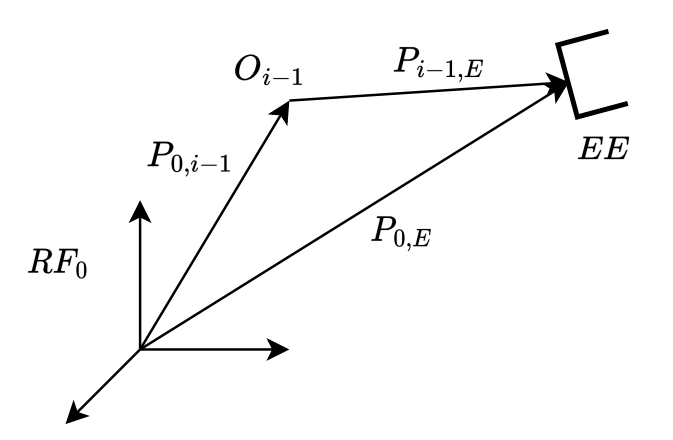
\includegraphics[width=0.75\linewidth]{PosizioneRelativaEE.png}
    \end{minipage}
\end{figure}

\newpage
\subsection{Analisi Della Mobilità Tramite Jacobiano} Fissata una specifica configurazione dei giunti $\bm{q}$, si può determinare quali movimenti l'end-effector può compiere istantaneamente. Quindi, Per una data configurazione, l'insieme di tutte le velocità che l'end-effector può assumere, è lo \textbf{Spazio Immagine} della matrice Jacobiana, indicato con $R(\bm{J})$. La dimensione di questo spazio, è definita dal rango della matrice, $\rho(\bm{J})$ e a seconda di questo valore possiamo trovarci in due situazioni distinte.

\paragraph{Configurazione Non-Singolare (Rango Pieno)}\mbox{}\\
Una configurazione è non-singolare quando il rango dello Jacobiano è massimo e coincide con la dimensione $m$ dello spazio di lavoro (con $m \le n$, dove $n$ è il numero di giunti). In questo caso, lo spazio delle velocità raggiungibili copre l'intero spazio di lavoro $\mathbb{R}^m$. e quindi il manipolatore gode della massima mobilità. Scegliendo opportunamente le velocità dei giunti, è possibile muovere l'end-effector istantaneamente in qualsiasi direzione desiderata.

\paragraph{Configurazione Singolare (Rango Deficiente)}\mbox{}\\
Una configurazione è singolare se il rango della Jacobiana è inferiore alla dimensione dello spazio di lavoro, ovvero $\rho(\bm{J}) < m$. In questa condizione, lo spazio delle velocità raggiungibili è un sottospazio proprio di $\mathbb{R}^m$ e quindi la mobilità del robot è limitata. Questo significa che esistono delle \textbf{direzioni di moto precluse}, ovvero delle velocità che l'end-effector è istantaneamente incapace di produrre, indipendentemente dalla velocità impressa ai giunti

\subsubsection{Identificare le Direzioni di Moto Precluse}
Attraverso la cinematica differenziale, lo Jacobiano mette in relazione le velocità dei giunti con le velocità lineari e angolari dell'end-effector. Si può scomporre lo spazio delle velocità dell'end-effector in due sottospazi ortogonali e complementari: lo spazio immagine dello Jacobiano $R(\bm{J})$, e lo spazio nullo della sua trasposta, $N(\bm{J}^T)$. Questa scomposizione, espressa dalla relazione:
\[
    \mathbb{R}^m = R(\bm{J}) \oplus N(\bm{J}^T)
\]
Questo significa che ogni vettore di velocità $\dot{\bm{r}}$ nello spazio di lavoro può essere visto unicamente come la somma di una componente in $R(\bm{J})$ e una in $N(\bm{J}^T)$.

Da ciò ne consegue una distinzione netta:
\begin{itemize}
    \item Le \textbf{Direzioni Di Moto Raggiungibili} sono tutte quelle che appartengono allo spazio immagine dello Jacobiano, $R(\bm{J})$. Questo sottospazio è generato dalle combinazioni lineari delle colonne $\bm{J}_{i}$ e rappresenta l'insieme di tutte le velocità che l'end-effector può generare a partire da una specifica configurazione del vettore delle variabili di giunto \(\bm{q}\)
    \item Le \textbf{Direzioni Di Moto Precluse}, sono le direzioni che si trovano nel nucleo della Jacobiana trasposta $N(\bm{J}^T)$. Questo sottospazio è ortogonale a $R(\bm{J})$ e contiene tutte le direzioni di velocità che l'end-effector non è in grado di eseguire in una data configurazione. In pratica, per trovare le direzioni in cui il movimento del robot è bloccato basta calcolare una base per il kernel di $\bm{J}^T$.
\end{itemize}

\subsubsection{Distinzione Fondamentale: Direzioni Precluse e Automovimenti}
È molto importante notare che il concetto di \textit{direzione di moto preclusa} è diverso dal concetto di \textit{automovimento}, in quanto sono due fenomeni diversi e appartengono a sottospazi differenenti.

\begin{itemize}
    \item \textbf{Direzioni di Moto Precluse ($N(\bm{J}^T)$):} Sono \textit{velocità dell'end-effector} che il robot non può fisicamente realizzare. Sono una \textbf{limitazione intrinseca} del manipolatore in una specifica configurazione.

    \item \textbf{Automovimenti ($N(\bm{J})$):} Sono \textit{velocità dei giunti} che, anche se fanno muovere la struttura del robot, \textbf{non producono una variazione della posa dell'end-effector} ($\dot{\bm{r}} = \bm{J}\dot{\bm{q}} = \bm{0}$). Rappresentano una \textbf{capacità aggiuntiva} del robot, tipica dei sistemi ridondanti. Un esempio pratico è la capacità di un braccio robotico con più di sei giunti di riposizionare il gomito per evitare una collisione, il tutto senza che la posa dell'end-effector cambi.
\end{itemize}

% \[
%     \dot{r} \quad       % Velocità
%     \ddot{r} \quad      % Accelerazione
%     \dddot{r} \quad     % Jerk
%     \ddddot{r}          % Snap
% \]

\newpage
\subsection{Esempio: Jacobiano Geometrico Del Robot Planare RR}
In questa sezione si applica il metodo sistematico per il calcolo del Jacobiano geometrico, uno strumento matematico fondamentale che mette in relazione le velocità dei giunti di un robot con le velocità lineari e angolari del suo end-effector. L'analisi è svolta per un robot planare a due giunti rotoidali (RR), come mostrato in figura.

\begin{minipage}[r]{0.25\textwidth}
    \centering
    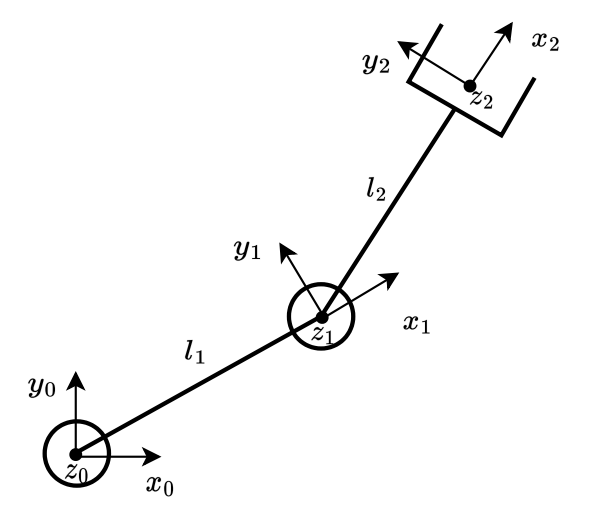
\includegraphics[width=0.99\linewidth]{RobotRRPlanare.png}
\end{minipage}
\hfill
\begin{minipage}[c]{0.73\textwidth}
Il primo passo consiste nel definire le matrici di trasformazione omogenea che descrivono la posizione e l'orientamento di ogni terna solidale ai bracci rispetto alla terna base. Utilizzando la convenzione di Denavit-Hartenberg, si ottengono le seguenti matrici. Per semplicità di notazione, si adotta la forma compatta \(c_i = \cos(q_i)\), \(s_i = \sin(q_i)\), \(c_{ij} = \cos(q_i + q_j)\) e \(s_{ij} = \sin(q_i + q_j)\).
    \[
        \;^{0}{\bm{T}}_0 = \bm{I}_{4 \times 4}
        \quad
        \;^{0}{\bm{T}}_1 =
        \begin{bmatrix}
            c_1 & -s_1 & 0 & l_1 c_1 \\
            s_1 & c_1 & 0 & l_1 s_1 \\
            0 & 0 & 1 & 0 \\
            0 & 0 & 0 & 1
        \end{bmatrix}
        \quad
        \;^{0}{\bm{T}}_2 =
        \begin{bmatrix}
            c_{12} & -s_{12} & 0 & l_1 c_1 + l_2 c_{12} \\
            s_{12} & c_{12} & 0 & l_1 s_1 + l_2 s_{12} \\
            0 & 0 & 1 & 0 \\
            0 & 0 & 0 & 1
        \end{bmatrix}
    \]
    Da queste matrici si estraggono i vettori necessari per costruire le colonne del Jacobiano.
\end{minipage}

Lo Jacobiano \(\bm{J}(\bm{q})\) è una matrice \(6 \times 2\) (poiché l'end-effector si muove nello spazio 3D e il robot ha 2 gradi di libertà) le cui colonne \( \bm{J}_i \) rappresentano il contributo del giunto \(i\)-esimo alla velocità dell'end-effector.

\paragraph{Calcolo Per La Colonna 1 (Giunto 1)}
La prima colonna del Jacobiano, \(\bm{J}_1\), descrive l'effetto della velocità del primo giunto, \(\dot{q}_1\), sulla velocità dell'end-effector. Poiché il giunto 1 è rotoidale, la sua colonna è data da:
\[ \bm{J}_1 = \begin{bmatrix} \bm{J}_{L1} \\ \bm{J}_{A1} \end{bmatrix} = \begin{bmatrix} \bm{z}_0 \times (\bm{p}_{0,e} - \bm{p}_{0,0}) \\ \bm{z}_0 \end{bmatrix} \]
dove \(\bm{z}_0\) è l'asse di rotazione del giunto 1 e \((\bm{p}_{0,e} - \bm{p}_{0,0})\) è il vettore "braccio di leva" che va dall'origine del giunto 1 all'end-effector.

\begin{itemize}
    \item \textbf{Asse di rotazione \(\bm{z}_0\):} Il primo giunto ruota attorno all'asse \(z\) della terna base (terna 0). Questo vettore è quindi per definizione:
    \[ \bm{z}_0 = \begin{bmatrix} 0 \\ 0 \\ 1 \end{bmatrix} \]
    \item \textbf{Vettore Leva \(\bm{p}_{0,e}\):} È il vettore posizione dell'end-effector rispetto alla terna base. Questo vettore si estrae direttamente dalla quarta colonna della matrice di trasformazione totale \(\;^{0}{\bm{T}}_2\). L'origine del giunto 1 coincide con l'origine della terna base, quindi \(\bm{p}_{0,0} = \bm{0}\) e il braccio di leva è semplicemente \(\bm{p}_{0,e}\).
    \[ \bm{p}_{0,e} = \begin{bmatrix} l_1 c_1 + l_2 c_{12} \\ l_1 s_1 + l_2 s_{12} \\ 0 \end{bmatrix} \]
\end{itemize}
Essendo un giunto rotoidale, si applicano le formule per calcolare la parte angolare (\(\bm{J}_{A1}\)) e lineare (\(\bm{J}_{L1}\)) della colonna:
\[
    \bm{J}_{A1} = \bm{z}_0 = \begin{bmatrix} 0 \\ 0 \\ 1 \end{bmatrix}
\]
La parte lineare si ottiene dal prodotto vettoriale tra l'asse di rotazione e il braccio di leva:
\[
    \bm{J}_{L1} = \bm{z}_0 \times \bm{p}_{0,e} =
    \begin{vmatrix}
        \bm{i} & \bm{j} & \bm{k} \\
        0 & 0 & 1 \\
        l_1 c_1 + l_2 c_{12} & l_1 s_1 + l_2 s_{12} & 0
    \end{vmatrix}
    = \begin{bmatrix} -(l_1 s_1 + l_2 s_{12}) \\ l_1 c_1 + l_2 c_{12} \\ 0 \end{bmatrix}
\]

\paragraph{Calcolo per la Colonna 2 (Giunto 2)}
La seconda colonna, \(\bm{J}_2\), descrive l'effetto della velocità del secondo giunto, \(\dot{q}_2\). La formula generale è:
\[ \bm{J}_2 = \begin{bmatrix} \bm{J}_{L2} \\ \bm{J}_{A2} \end{bmatrix} = \begin{bmatrix} \bm{z}_1 \times (\bm{p}_{0,e} - \bm{p}_{0,1}) \\ \bm{z}_1 \end{bmatrix} \]
dove \(\bm{z}_1\) è l'asse di rotazione del giunto 2 e \((\bm{p}_{0,e} - \bm{p}_{0,1})\) è il vettore che congiunge l'origine del giunto 2 con l'end-effector.

\begin{itemize}
    \item \textbf{Asse di rotazione \(\bm{z}_1\):} È l'asse di rotazione del secondo giunto, espresso nelle coordinate della terna base. Si ottiene estraendo la terza colonna della matrice di rotazione \(\prescript{0}{}{\bm{R}}_1\), che è la sottomatrice \(3 \times 3\) in alto a sinistra di \(\prescript{0}{}{\bm{T}}_1\). In questo caso planare, l'asse di rotazione è sempre parallelo all'asse \(z\) globale.
    \[ \bm{z}_1 = \begin{bmatrix} 0 \\ 0 \\ 1 \end{bmatrix} \]
    \item \textbf{Vettore Leva \(\bm{p}_{1,e}\):} È il vettore che va dall'origine del giunto 2 all'end-effector, calcolato come \(\bm{p}_{1,e} = \bm{p}_{0,e} - \bm{p}_{0,1}\). Il vettore \(\bm{p}_{0,1}\) (posizione del giunto 2 rispetto alla base) si trova nella quarta colonna di \(\prescript{0}{}{\bm{T}}_1\).
    \[
        \bm{p}_{1,e} =
        \begin{bmatrix} l_1 c_1 + l_2 c_{12} \\ l_1 s_1 + l_2 s_{12} \\ 0 \end{bmatrix}
        -
        \begin{bmatrix} l_1 c_1 \\ l_1 s_1 \\ 0 \end{bmatrix}
        =
        \begin{bmatrix} l_2 c_{12} \\ l_2 s_{12} \\ 0 \end{bmatrix}
    \]
\end{itemize}
Anche il secondo giunto è rotoidale, quindi si usano le stesse formule:
\[
    \bm{J}_{A2} = \bm{z}_1 = \begin{bmatrix} 0 \\ 0 \\ 1 \end{bmatrix}
\]
\[
    \bm{J}_{L2} = \bm{z}_1 \times \bm{p}_{1,e} =
    \begin{vmatrix}
        \bm{i} & \bm{j} & \bm{k} \\
        0 & 0 & 1 \\
        l_2 c_{12} & l_2 s_{12} & 0
    \end{vmatrix}
    = \begin{bmatrix} -l_2 s_{12} \\ l_2 c_{12} \\ 0 \end{bmatrix}
\]

\paragraph{Jacobiano Geometrico Completo}\(\mbox{}\)\\
Assemblando le colonne calcolate, si ottiene lo Jacobiano geometrico completo. La matrice è strutturata con la parte relativa alla velocità lineare (\(\bm{J}_L\)) nelle prime tre righe e quella relativa alla velocità angolare (\(\bm{J}_A\)) nelle ultime tre.
\[
    \bm{J}(\bm{q}) =
    \begin{bmatrix}
        \bm{J}_{L1} & \bm{J}_{L2} \\
        \bm{J}_{A1} & \bm{J}_{A2}
    \end{bmatrix}
    =
    \begin{bmatrix}
        -l_1 s_1 - l_2 s_{12} & -l_2 s_{12} \\
        l_1 c_1 + l_2 c_{12} & l_2 c_{12} \\
        0 & 0 \\
        \hdashline[2pt/2pt]
        0 & 0 \\
        0 & 0 \\
        1 & 1
    \end{bmatrix}
\]
La relazione tra le velocità dei giunti \(\dot{\bm{q}} = [\dot{q}_1, \dot{q}_2]^T\) e le velocità dell'end-effector \(\bm{\dot{r}}_e = [\bm{v}_e^T, \bm{\omega}_e^T]^T\) è data da \(\bm{\dot{r}}_e = \bm{J}(\bm{q})\dot{\bm{q}}\). Espandendo questa equazione, si ottengono le espressioni per la velocità lineare \(\bm{v}_e\) e angolare \(\bm{\omega}_e\):
\[
    \bm{v}_e =
    \begin{bmatrix} -l_1 s_1 - l_2 s_{12} \\ l_1 c_1 + l_2 c_{12} \\ 0 \end{bmatrix} \dot{q}_1
    +
    \begin{bmatrix} -l_2 s_{12} \\ l_2 c_{12} \\ 0 \end{bmatrix} \dot{q}_2
\]
\[
    \bm{\omega}_e =
    \begin{bmatrix} 0 \\ 0 \\ 1 \end{bmatrix} \dot{q}_1
    +
    \begin{bmatrix} 0 \\ 0 \\ 1 \end{bmatrix} \dot{q}_2
    = \begin{bmatrix} 0 \\ 0 \\ \dot{q}_1 + \dot{q}_2 \end{bmatrix}
\]
Queste equazioni mostrano esplicitamente come la velocità di ciascun giunto contribuisca al moto dell'organo terminale. La velocità angolare totale, ad esempio, è semplicemente la somma delle velocità angolari dei due giunti, come è logico attendersi in un sistema planare.

\newpage
\subsection{Relazione tra Singolarità e Jacobiano}
\subsubsection{Richiami di Algebra Lineare}

La matrice Jacobiana \(\bm{J}\) è lo strumento matematico che crea un ponte tra lo spazio delle velocità dei giunti e lo spazio delle velocità dell'end-effector, secondo la relazione \(\bm{\dot{r}} = \bm{J}(\bm{q})\dot{\bm{q}}\). Le configurazioni in cui un robot perde la capacità di muoversi in certe direzioni, note come singolarità, sono interamente descritte dalle proprietà algebriche della matrice Jacobiana. Analizziamo i concetti fondamentali.

\begin{itemize}
    \item \textbf{Rango di una Matrice:} Data una matrice $\bm{J} \in \mathbb{R}^{m \times n}$, il suo \textit{rango}, denotato con $\rho(\bm{J})$, è il massimo numero di colonne (o righe) linearmente indipendenti. Fisicamente, il rango rappresenta il numero di direzioni indipendenti lungo le quali l'end-effector può muoversi (sia in traslazione che in rotazione). Il rango è sempre limitato dalla dimensione più piccola della matrice:
    \[
        \rho(\bm{J}) \leq \min\{m, n\}
    \]

    \item \textbf{Rango Pieno e Rango Carente:} Si dice che la matrice \(\bm{J}\) ha \textit{rango pieno} quando il suo rango raggiunge il valore massimo possibile, ovvero $\rho(\bm{J}) = \min\{m, n\}$. In questa condizione, il robot ha la massima manovrabilità possibile per la sua struttura. Se, in una certa configurazione \(\bm{q}\), il rango diminuisce, $\rho(\bm{J}) < \min\{m, n\}$, si dice che la matrice è \textit{rango-carente} (o \textit{rank-deficient}), e il robot si trova in una \textbf{singolarità}.

    \item \textbf{Matrice Singolare e Non-Singolare (per matrici quadrate):} Nel caso comune di robot non ridondanti, dove il numero di giunti \(n\) è uguale al numero di gradi di libertà dell'end-effector \(m\), lo Jacobiano è una matrice quadrata ($\bm{J} \in \mathbb{R}^{n \times n}$).
    \begin{itemize}
        \item Una matrice quadrata è detta \textbf{non-singolare} se ha rango pieno ($\rho(\bm{J}) = n$). Questa condizione è equivalente ad affermare che il suo determinante è non nullo ($\det(\bm{J}) \neq 0$) e che esiste la sua unica matrice inversa $\bm{J}^{-1}$, tale che $\bm{J}\bm{J}^{-1} = \bm{J}^{-1}\bm{J} = \bm{I}$. L'invertibilità è cruciale: permette di calcolare in modo univoco le velocità dei giunti \(\dot{\bm{q}}\) necessarie per ottenere una data velocità dell'end-effector \(\bm{\dot{r}}\) tramite la relazione \(\dot{\bm{q}} = \bm{J}^{-1}\bm{\dot{r}}\).
        \item Una matrice quadrata è detta \textbf{singolare} se non è invertibile. Ciò accade precisamente quando la matrice è rango-carente ($\rho(\bm{J}) < n$), ovvero quando il suo determinante è nullo. In una configurazione singolare, il robot perde uno o più gradi di libertà e non è più possibile mappare univocamente le velocità cartesiane a quelle dei giunti.
    \end{itemize}

    \item \textbf{Immagine (o Spazio delle Colonne):} L'\textit{immagine} di \(\bm{J}\), indicata con $R(\bm{J})$, è il sottospazio vettoriale generato dalle colonne di \(\bm{J}\). In termini pratici, rappresenta l'insieme di \textbf{tutte le possibili velocità dell'end-effector} \(\bm{\dot{r}}\) che il robot può generare.
    \[
        R(\bm{J}) = \{\bm{\dot{r}} \in \mathbb{R}^{m} \mid \exists \dot{\bm{q}} \in \mathbb{R}^{n} \text{ tale che } \bm{\dot{r}} = \bm{J}\dot{\bm{q}}\}
    \]
    La dimensione di questo sottospazio è esattamente il rango della matrice:
    \[
        \dim(R(\bm{J})) = \rho(\bm{J})
    \]
    Quando il robot entra in una singolarità, il rango \(\rho(\bm{J})\) diminuisce, e con esso si "restringe" lo spazio delle velocità raggiungibili dall'end-effector.

    \item \textbf{Nucleo (o Spazio Nullo):} Il \textit{nucleo} di \(\bm{J}\), indicato con $N(\bm{J})$, è il sottospazio dei vettori di velocità dei giunti \(\dot{\bm{q}}\) che producono una velocità nulla dell'end-effector.
    \[
        N(\bm{J}) = \{\dot{\bm{q}} \in \mathbb{R}^{n} \mid \bm{J}\dot{\bm{q}} = \bm{0}\}
    \]
    Un nucleo non banale (cioè che non contiene solo il vettore nullo) implica l'esistenza di \textbf{movimenti interni} dei giunti che non modificano la posa dell'end-effector. Questo fenomeno è la base della \textbf{ridondanza} nei robot.
    \newpage
    \item \textbf{Teorema Rango-Nullità:} Questo teorema fondamentale lega le dimensioni dell'immagine e del nucleo al numero di giunti \(n\) (la dimensione dello spazio di partenza):
    \[
        \dim(R(\bm{J})) + \dim(N(\bm{J})) = n
    \]
    Sostituendo $\dim(R(\bm{J})) = \rho(\bm{J})$, si ottiene:
    \[
        \dim(N(\bm{J})) = n - \rho(\bm{J})
    \]
    Questa relazione ci dice che se il rango diminuisce (singolarità), la dimensione dello spazio nullo aumenta. Anche per un robot non ridondante, in una singolarità compare un nucleo non banale, che si manifesta come un moto istantaneo dei giunti che non produce movimento dell'end-effector.

    \item \textbf{Sottospazi Fondamentali e Decomposizione Ortogonale:} Per una comprensione completa della trasformazione operata da \(\bm{J}\), si analizzano i quattro sottospazi fondamentali: l'immagine \(R(\bm{J})\), il nucleo \(N(\bm{J})\), e i corrispondenti spazi per la sua trasposta, \(R(\bm{J}^T)\) e \(N(\bm{J}^T)\). Questi sottospazi permettono di decomporre gli spazi di partenza (velocità dei giunti, \(\mathbb{R}^n\)) e di arrivo (velocità dell'end-effector, \(\mathbb{R}^m\)) in componenti ortogonali.
    \[
    \begin{cases}
        R(\bm{J}) \oplus N(\bm{J}^T) = \mathbb{R}^{m} \\
        R(\bm{J}^T) \oplus N(\bm{J}) = \mathbb{R}^{n}
    \end{cases}
    \]
    Il simbolo \(\oplus\) denota la \textit{somma diretta}, che implica che ogni vettore dello spazio può essere scritto in modo \textbf{unico} come somma di un vettore da ciascun sottospazio.

    La seconda relazione, $R(\bm{J}^T) \oplus N(\bm{J}) = \mathbb{R}^{n}$, è particolarmente significativa:
    \begin{itemize}
        \item Lo spazio \(R(\bm{J}^T)\) è l'insieme delle velocità dei giunti che sono "efficienti", ovvero che producono un movimento dell'end-effector.
        \item Lo spazio \(N(\bm{J})\) è l'insieme delle velocità dei giunti che corrispondono a moti interni (inefficienti dal punto di vista del movimento dell'end-effector).
    \end{itemize}
    Questa decomposizione ci dice che qualsiasi vettore di velocità dei giunti \(\dot{\bm{q}}\) può essere scomposto in modo univoco in una componente che muove l'end-effector e una che non lo fa.
\end{itemize}


\newpage
\subsection{Spazio Dei Giunti E Spazio Dei Compiti}
Nell'analisi cinematica è fondamentale la matrice Jacobiana, indicata con $\bm{J}$, che non è una matrice costante. Infatti, dipende dalla configurazione del robot, la quale è descritta dal vettore delle variabili di giunto $\bm{q}$. Questa dipendenza implica che tutte le proprietà fondamentali dello Jacobiano come il rango $\rho$, lo spazio immagine $R$, e il nucleo $N$ siano proprietà \textit{locali}, che variano al variare di $\bm{q}$:
\[
    \rho(\bm{J}) = \rho(\bm{J}(\bm{q})), \quad R(\bm{J}) = R(\bm{J}(\bm{q})), \quad N(\bm{J}) = N(\bm{J}(\bm{q}))
\]
La relazione cinematica differenziale, espressa dall'equazione $\bm{v} = \bm{J}(\bm{q})\dot{\bm{q}}$, fornisce la chiave per dare un'interpretazione fisica diretta a questi sottospazi matematici.

\begin{center}
    \resizebox{0.75\linewidth}{!}{%
        \begin{tikzpicture}
            % Cerchio centrato in un punto
            \draw (2,2) circle (1.75cm);
            \draw (2,2) circle (1cm);

            \draw (10,2) circle (1.75cm);
            \draw (10,2) circle (1cm);

            % Punto definito con coordinate
            \filldraw[black] (1.75,2.25) circle (1.5pt);
            \node at (1.75,2.5) {$\bm{0}$};

            \filldraw[black] (10,2.25) circle (1.5pt);
            \node at (10,2.5) {$\bm{0}$};

            % Linea che collega due punti
            \draw (2, 3.75) -- (10, 3);
            \draw (2, 0.25) -- (10, 1);

            \draw (2, 3) -- (10,2.25);
            \draw (2, 1) -- (10,2.25);

            % Etichette
            \node at (2,1.5) {$N(J)$};
            \node at (10,1.5) {$R(J)$};
        \end{tikzpicture}
    }
\end{center}

\begin{itemize}
    \item \textbf{Spazio Velocità Raggiungibili:} Lo spazio immagine dello Jacobiano, $R(\bm{J}(\bm{q}))$, noto anche come \textit{spazio delle velocità generalizzate}, rappresenta l'intero insieme di velocità (sia lineari che angolari) che l'end-effector è in grado di raggiungere in una specifica configurazione $\bm{q}$. Questo spazio si ottiene considerando tutte le possibili combinazioni di velocità dei giunti $\dot{\bm{q}}$. Quando il rango della matrice è massimo e coincide con la dimensione dello spazio dei compiti ($m$), ovvero $\rho(\bm{J}(\bm{q})) = m$, il robot gode della massima manovrabilità e quindi l'end-effector può muoversi istantaneamente in qualsiasi direzione dello spazio operativo $\mathbb{R}^{m}$.

    \item \textbf{Direzioni Di Moto Precluse:} Quando, in una data configurazione $\bm{q}$, il rango dello Jacobiano scende al di sotto della dimensione dello spazio dei compiti ($\rho(\bm{J}(\bm{q})) < m$), emergono delle limitazioni. In queste condizioni, esistono delle direzioni nello spazio operativo $\mathbb{R}^{m}$ lungo le quali l'end-effector non può muoversi, indipendentemente dalla velocità dei giunti. Queste direzioni "proibite" sono definite dal sottospazio $N(\bm{J}^T(\bm{q}))$. Una configurazione che presenta questa perdita di mobilità è definita \textit{configurazione singolare} o, più semplicemente, \textit{singolarità}.

    \item \textbf{Automovimenti:} Se lo spazio nullo dello Jacobiano, $N(\bm{J}(\bm{q}))$, non è banale, cioè se contiene vettori non nulli, allora è fisicamente possibile avere combinazioni di velocità dei giunti non nulle ($\dot{\bm{q}} \neq \bm{0}$) che producono una velocità dell'end-effector pari a zero ($\bm{v} = \bm{0}$). Questi movimenti, che modificano la configurazione interna del robot senza spostare l'end-effector, sono chiamati \textit{automovimenti}. Questa caratteristica è tipica dei \textit{robot ridondanti}, ovvero quei robot in cui il numero di giunti è maggiore della dimensione dello spazio dei compiti ($n > m$). Per tali sistemi, la condizione $N(\bm{J}(\bm{q})) \neq \{\bm{0}\}$ è sempre verificata.
\end{itemize}

\newpage
\subsection{Analisi della Mobilità nello Spazio dei Compiti: Robot RRR Planare}
Si consideri un manipolatore planare composto da tre giunti rotoidali (configurazione RRR). Per semplificare i calcoli, assumiamo che tutti i bracci abbiano la stessa lunghezza, pari a uno: $l_1 = l_2 = l_3 = 1$.

Il compito che vogliamo assegnare a questo robot è il controllo della \textbf{posizione} dell' end-effector nel piano $xy$. Tale posizione è descritta dal vettore $\bm{r} = [x, y]^T$. Lo spazio in cui il compito è definito (lo "spazio dei compiti") ha quindi dimensione $m=2$. D'altra parte, il robot è descritto da tre variabili di giunto indipendenti ($q_1, q_2, q_3$), per cui il suo spazio di configurazione (o "spazio dei giunti") ha dimensione $n=3$.

Poiché il numero di gradi di libertà del robot ($n=3$) è maggiore del numero di gradi di libertà richiesti per eseguire il compito ($m=2$), il robot è definito \textbf{ridondante} rispetto a questo specifico compito. Ciò significa che esistono infinite configurazioni dei giunti che permettono all'end-effector di raggiungere la stessa posizione nel piano.

Lo spazio di lavoro del manipolatore, ovvero l'insieme di tutti i punti raggiungibili dall'end-effector, è una corona circolare. Il raggio esterno di 3 (unità) si ottiene quando tutti i bracci sono completamente estesi in linea retta, mentre il raggio interno di 1 (unità) si ha quando il secondo e il terzo braccio sono ripiegati sul primo.

\begin{figure}[h!]
    \centering
    \begin{minipage}[b]{0.45\textwidth}
        \centering
        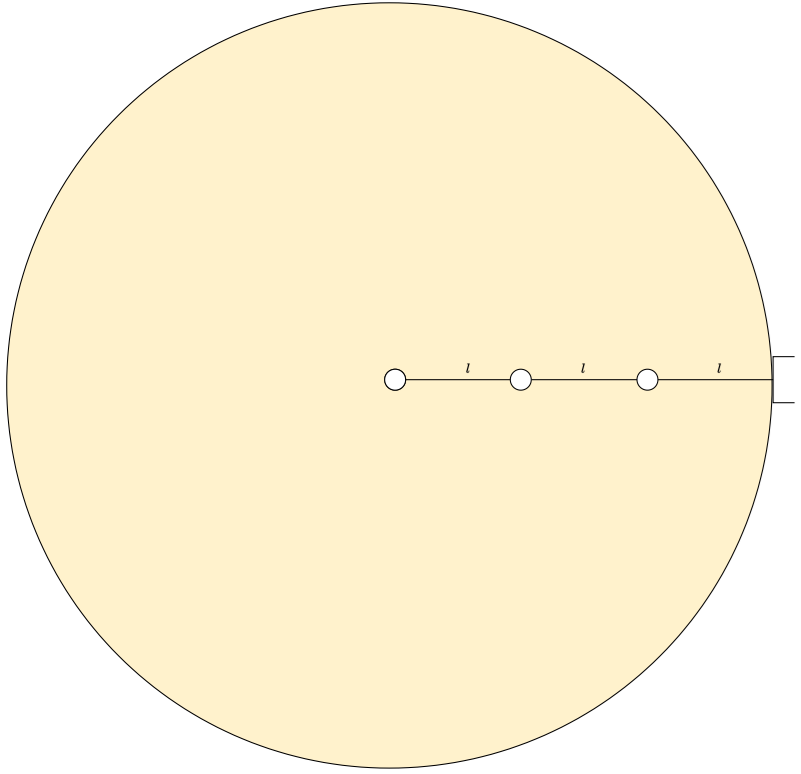
\includegraphics[width=0.7\linewidth]{SpazioOperativoPrimario.png}
        \caption{Spazio Operativo Primario (Raggio 3)}
    \end{minipage}
    \hfill
    \begin{minipage}[b]{0.45\textwidth}
        \centering
        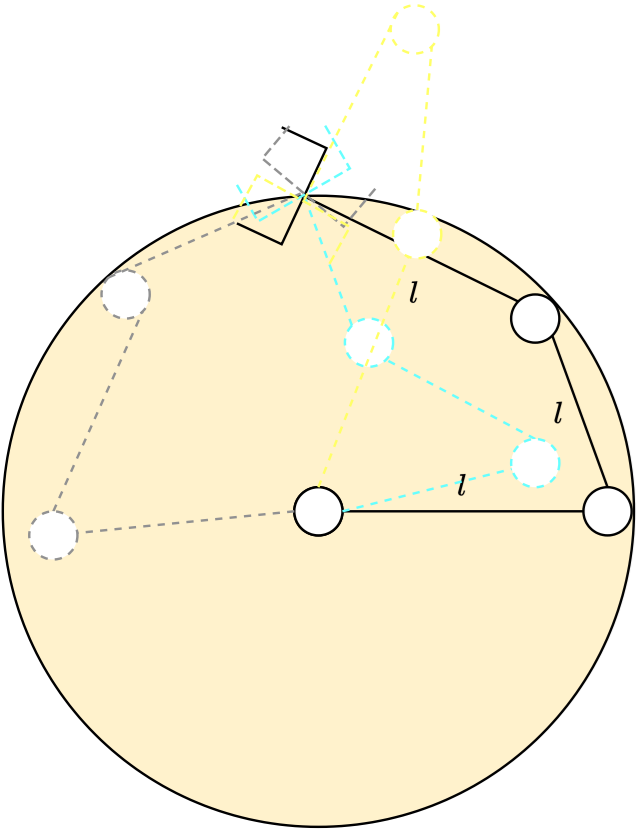
\includegraphics[width=0.65\linewidth]{SpazioOperativoSecondario.png}
        \caption{Spazio Operativo Secondario (Raggio 1)}
    \end{minipage}
\end{figure}

\paragraph{Passo 1: Cinematica Diretta e Matrici di Trasformazione.}
Il primo passo per poter analizzare la mobilità del robot è derivare il suo modello cinematico diretto. Come sappiamo, si deve calcolare la funzione matematica che ci fornisce la posizione (e l'orientamento) dell'end-effector a partire da una data configurazione del vettore delle variabili di giunto $\bm{q} = [q_1, q_2, q_3]^T$. Per ottenere questo modello, utilizziamo la \textbf{convenzione di Denavit-Hartenberg (DH)}. I parametri DH per il nostro manipolatore RRR planare sono riportati nella tabella:.

\begin{table}[h!]
    \centering
    \begin{tabular}{|c|cccc|}
        \hline
        \textbf{Braccio} & $\boldsymbol{\theta_i}$ & $\boldsymbol{d_i}$ & $\boldsymbol{\alpha_i}$ & $\boldsymbol{a_i}$ \\
        \hline
        1 & $q_{1}$ & 0 & 0 & $l_1=1$ \\
        2 & $q_{2}$ & 0 & 0 & $l_2=1$ \\
        3 & $q_{3}$ & 0 & 0 & $l_3=1$ \\
        \hline
    \end{tabular}
\end{table}

Sostituendo questi parametri nella matrice di trasformazione omogenea standard, si ottengono le matrici che descrivono la posa (posizione e orientamento) di ogni terna di riferimento solidale a un braccio rispetto alla terna precedente.
\newpage
Data la semplicità della cinematica planare e la scelta dei parametri DH, le matrici sono:
\[
    {}^0\bm{A}_1(q_1) =
    \begin{bmatrix}
        c_1 & -s_1 & 0 & c_1 \\
        s_1 & c_1 & 0 & s_1 \\
        0 & 0 & 1 & 0 \\
        0 & 0 & 0 & 1
    \end{bmatrix} \! , \quad
    {}^1\bm{A}_2(q_2) =
    \begin{bmatrix}
        c_2 & -s_2 & 0 & c_2 \\
        s_2 & c_2 & 0 & s_2 \\
        0 & 0 & 1 & 0 \\
        0 & 0 & 0 & 1
    \end{bmatrix} \! , \quad
    {}^2\bm{A}_3(q_3) =
    \begin{bmatrix}
        c_3 & -s_3 & 0 & c_3 \\
        s_3 & c_3 & 0 & s_3 \\
        0 & 0 & 1 & 0 \\
        0 & 0 & 0 & 1
    \end{bmatrix}
\]
Dove, per compattezza, si adotta la notazione $c_i = \cos(q_i)$ e $s_i = \sin(q_i)$.

La posa completa dell'end-effector (terna $\{3\}$) rispetto alla base del robot (terna $\{0\}$) si ottiene componendo queste trasformazioni, ovvero moltiplicando le matrici singole: ${}^0\bm{A}_3(\bm{q}) = {}^0\bm{A}_1(q_1) {}^1\bm{A}_2(q_2) {}^2\bm{A}_3(q_3)$. Il risultato di questo prodotto è:
\[
    {}^0\bm{A}_3(\bm{q}) =
    \begin{bmatrix}
        c_{123} & -s_{123} & 0 & c_1 + c_{12} + c_{123} \\
        s_{123} & c_{123} & 0 & s_1 + s_{12} + s_{123} \\
        0 & 0 & 1 & 0 \\
        0 & 0 & 0 & 1
    \end{bmatrix}
\]
Dove si è usata la notazione $c_{12} = \cos(q_1+q_2)$, $s_{123} = \sin(q_1+q_2+q_3)$. La quarta colonna di questa matrice rappresenta il vettore posizione dell'origine della terna $\{3\}$ rispetto alla terna $\{0\}$. Poiché il nostro compito riguarda solo la posizione planare, estraiamo le prime due componenti di questo vettore per ottenere la funzione di cinematica diretta che ci interessa:
\[
    \bm{r}(\bm{q}) =
    \begin{bmatrix} x(\bm{q}) \\ y(\bm{q}) \end{bmatrix} =
    \begin{bmatrix}
        c_1 + c_{12} + c_{123} \\
        s_1 + s_{12} + s_{123}
    \end{bmatrix}
\]

\paragraph{Passo 2: Calcolo del Jacobiano Geometrico.}
Lo Jacobiano è una matrice che lega le velocità nello spazio dei giunti ($\dot{\bm{q}}$) alle velocità nello spazio dei compiti. In particolare, il \textbf{Jacobiano geometrico} $\bm{J}(\bm{q}) \in \mathbb{R}^{6 \times 3}$ mappa le velocità angolari dei tre giunti alla velocità spaziale dell'end-effector, composta da un vettore di velocità lineare $\bm{v} \in \mathbb{R}^3$ e un vettore di velocità angolare $\bm{\omega} \in \mathbb{R}^3$.

La sua struttura si costruisce colonna per colonna, dove ogni colonna $\bm{J}_i$ rappresenta il contributo del giunto $i$-esimo alla velocità dell'end-effector. Per i giunti rotoidali, la formula è:
\[
\bm{J}_i =
\begin{bmatrix} \bm{J}_{Li} \\ \bm{J}_{Ai} \end{bmatrix} =
\begin{bmatrix} \bm{z}_{i-1} \times (\bm{p}_E - \bm{p}_{i-1}) \\ \bm{z}_{i-1} \end{bmatrix}
\]
Dove:
\begin{itemize}
    \item $\bm{z}_{i-1}$: È il versore che indica l'asse di rotazione del giunto $i$.
    \item $(\bm{p}_E - \bm{p}_{i-1})$: È il vettore che va dall'origine del giunto $i$ alla punta dell'end-effector (il "braccio di leva").
\end{itemize}

Dato che il nostro è un robot planare, tutti i giunti ruotano attorno ad assi paralleli all'asse $z$ del sistema di riferimento base. Pertanto, i vettori degli assi di rotazione sono costanti e uguali:
\[
    \bm{z}_0 = \bm{z}_1 = \bm{z}_2 = \begin{bmatrix} 0 & 0 & 1 \end{bmatrix}^T
\]
Per calcolare i vettori "braccio di leva", dobbiamo trovare le posizioni delle origini dei sistemi di riferimento di ciascun giunto ($\bm{p}_0, \bm{p}_1, \bm{p}_2$) e la posizione dell'end-effector ($\bm{p}_E$). Queste possono essere estratte dalle matrici di trasformazione parziali:
\[
\begin{aligned}
    % Leva Giunto 1
    \bm{p}_{0,E} &= \bm{p}_E - \bm{p}_0 = \begin{bmatrix} x \\ y \\ 0 \end{bmatrix} - \begin{bmatrix} 0 \\ 0 \\ 0 \end{bmatrix} = \begin{bmatrix} c_1+c_{12}+c_{123} \\ s_1+s_{12}+s_{123} \\ 0 \end{bmatrix} \\
    % Leva Giunto 2
    \bm{p}_{1,E} &= \bm{p}_E - \bm{p}_1 = \begin{bmatrix} x \\ y \\ 0 \end{bmatrix} - \begin{bmatrix} c_1 \\ s_1 \\ 0 \end{bmatrix} = \begin{bmatrix} c_{12}+c_{123} \\ s_{12}+s_{123} \\ 0 \end{bmatrix} \\
    % Leva Giunto 3
    \bm{p}_{2,E} &= \bm{p}_E - \bm{p}_2 = \begin{bmatrix} x \\ y \\ 0 \end{bmatrix} - \begin{bmatrix} c_1+c_{12} \\ s_1+s_{12} \\ 0 \end{bmatrix} = \begin{bmatrix} c_{123} \\ s_{123} \\ 0 \end{bmatrix}
\end{aligned}
\]
Procediamo ora con il calcolo esplicito delle colonne del Jacobiano tramite il prodotto vettoriale:
\[
\begin{alignedat}{2}
    % Colonna 1
    \bm{J}_{L1} &= \bm{z}_0 \times \bm{p}_{0,E} = \begin{bmatrix} -(s_1+s_{12}+s_{123}) \\ c_1+c_{12}+c_{123} \\ 0 \end{bmatrix} &\quad \bm{J}_{A1} &= \bm{z}_0 = \begin{bmatrix} 0 \\ 0 \\ 1 \end{bmatrix} \\
    % Colonna 2
    \bm{J}_{L2} &= \bm{z}_1 \times \bm{p}_{1,E} = \begin{bmatrix} -(s_{12}+s_{123}) \\ c_{12}+c_{123} \\ 0 \end{bmatrix} &\quad \bm{J}_{A2} &= \bm{z}_1 = \begin{bmatrix} 0 \\ 0 \\ 1 \end{bmatrix} \\
    % Colonna 3
    \bm{J}_{L3} &= \bm{z}_2 \times \bm{p}_{2,E} = \begin{bmatrix} -s_{123} \\ c_{123} \\ 0 \end{bmatrix} &\quad \bm{J}_{A3} &= \bm{z}_2 = \begin{bmatrix} 0 \\ 0 \\ 1 \end{bmatrix}
\end{alignedat}
\]
Assemblando queste colonne, otteniamo lo Jacobiano geometrico completo $6 \times 3$:
\[
    \bm{J}(\bm{q}) =
    \begin{bmatrix}
        % Righe velocità lineari (vx, vy, vz)
        -(s_{1} + s_{12} + s_{123}) & -(s_{12} + s_{123}) & -s_{123} \\
        c_{1} + c_{12} + c_{123} & c_{12} + c_{123} & c_{123} \\
        0 & 0 & 0 \\
        \hline
        % Righe velocità angolari (wx, wy, wz)
        0 & 0 & 0 \\
        0 & 0 & 0 \\
        1 & 1 & 1
    \end{bmatrix}
\]

\paragraph{Passo 3: Dal Jacobiano Geometrico al Jacobiano Analitico}
Lo Jacobiano geometrico descrive l'intera velocità spaziale dell'end-effector. Tuttavia, il nostro compito è stato definito in modo più semplice: controllare solo la posizione planare $\bm{r} = [x, y]^T$. Non siamo interessati né alla velocità lungo l'asse $z$ (che è sempre nulla per un robot planare), né alla velocità angolare.

Pertanto, per i nostri scopi, possiamo estrarre dallo Jacobiano geometrico solo le righe che ci interessano, ovvero quelle che corrispondono alle velocità $\dot{x}$ (prima riga) e $\dot{y}$ (seconda riga). Questo processo ci fornisce lo \textbf{Jacobiano di Posizione} $\bm{J}_r(\bm{q}) \in \mathbb{R}^{2 \times 3}$, una matrice che lega direttamente le velocità dei giunti alla velocità cartesiana dell'end-effector nel piano, secondo la relazione fondamentale: $\dot{\bm{r}} = \bm{J}_r(\bm{q})\dot{\bm{q}}$.

Vale la pena notare che si sarebbe potuto ottenere lo stesso risultato derivando direttamente la funzione di posizione $\bm{r}(\bm{q})$ rispetto al vettore dei giunti $\bm{q}$:
\[
    \bm{J}_r(\bm{q}) = \frac{\partial \bm{r}(\bm{q})}{\partial \bm{q}} =
    \begin{bmatrix}
        \frac{\partial x}{\partial q_1} & \frac{\partial x}{\partial q_2} & \frac{\partial x}{\partial q_3} \\
        \frac{\partial y}{\partial q_1} & \frac{\partial y}{\partial q_2} & \frac{\partial y}{\partial q_3}
    \end{bmatrix}
    =
    \begin{bmatrix}
        -(s_{1} + s_{12} + s_{123}) & -(s_{12} + s_{123}) & -s_{123} \\
        c_{1} + c_{12} + c_{123} & c_{12} + c_{123} & c_{123}
    \end{bmatrix}
\]
Questa matrice finale, di dimensioni $2 \times 3$, è lo strumento analitico cruciale che ci permetterà di studiare le configurazioni singolari del robot. Le singolarità si verificano in quelle configurazioni di giunti $\bm{q}$ in cui il rango di $\bm{J}_r$ scende al di sotto del suo valore massimo (che in questo caso è 2), indicando che il robot perde la capacità di muovere il suo end-effector in una o più direzioni del piano.

\newpage
\paragraph{Analisi di Caso 1: Robot Ripiegato (Configurazione Non Singolare)}
\mbox{}\\ % Forza l'inizio di una nuova linea
Per comprendere il significato pratico del Jacobiano, iniziamo analizzando una configurazione specifica e intuitivamente robusta: $\bm{q}_1 = [0, \pi/2, -\pi/2]^T$. Come mostra la figura, in questa posa il robot è parzialmente ripiegato su se stesso, lontano dai limiti del suo spazio di lavoro.

\begin{minipage}[b]{0.33\textwidth}
    \centering
    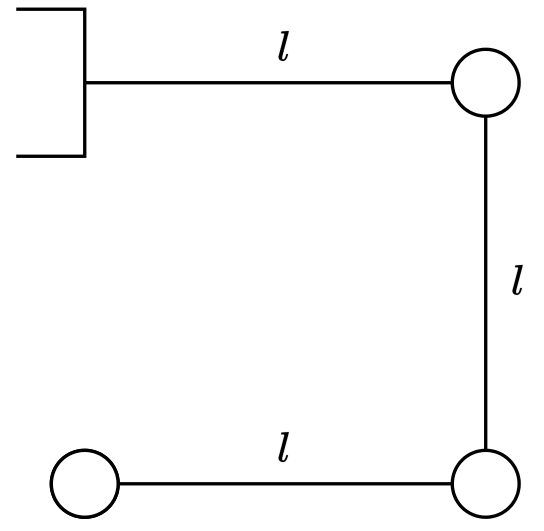
\includegraphics[width=0.75\linewidth]{ConfigurazioneQ1.png}
\end{minipage}
\hfill
\begin{minipage}[b]{0.65\textwidth}
    Per prima cosa, calcoliamo lo Jacobiano in questa configurazione sostituendo i valori degli angoli nella matrice $\bm{J}_r(\bm{q})$ che abbiamo derivato in precedenza. Otteniamo:
    \[
        \bm{J}_r(\bm{q}_1) =
        \begin{bmatrix}
            -1 & -1 & 0 \\
            0 & -1 & -1
        \end{bmatrix}
    \]
\end{minipage}

L'analisi algebrica di questa matrice ci fornisce un quadro completo della mobilità del robot.

\subparagraph{Rango e Spazio Immagine (Direzioni Moto Possibili)}
Il rango della matrice \(\bm{J}_r(\bm{q}_i)\) ci dice quante direzioni indipendenti può generare e siccome è una matrice $2 \times 3$, il rango massimo è 2. Osservando $\bm{J}_r(\bm{q}_1)$, si nota che le prime due colonne, $\begin{bmatrix}-1 \\ 0\end{bmatrix}$ e $\begin{bmatrix}-1 \\ -1\end{bmatrix}$, non sono proporzionali, e quindi sono linearmente indipendenti. Questo è sufficiente per affermare che il rango della matrice è il massimo possibile: $\rho(\bm{J}_r(\bm{q}_1)) = 2$.

Poiché il rango è uguale alla dimensione dello spazio del compito ($m=2$), la matrice ha \textbf{rango pieno}. Questo, per definizione, significa che la configurazione \textbf{non è singolare}.
Lo spazio immagine $R(\bm{J}_r(\bm{q}_1))$, che è l'insieme di tutte le velocità dell'end-effector che possono essere generate, è lo spazio generato dalle colonne della matrice. Poiché abbiamo due colonne linearmente indipendenti in uno spazio 2D, esse generano l'intero piano:
\[
    R(\bm{J}_r(\bm{q}_1)) = \mathrm{span}\left\{
    \begin{bmatrix} -1 \\ 0 \end{bmatrix},
    \begin{bmatrix} -1 \\ -1 \end{bmatrix},
    \begin{bmatrix} 0 \\ -1 \end{bmatrix}
    \right\} = \mathbb{R}^{2}
\]
In questa configurazione, il robot gode della massima mobilità. Qualunque direzione di movimento si desideri per l'end-effector nel piano, esiste una combinazione di velocità dei giunti in grado di produrla.

\subparagraph{Nucleo e Automovimenti (Moti Interni).}
Poiché il robot è ridondante ($n=3 > m=2$), ci aspettiamo di poter muovere i giunti senza che l'end-effector si sposti. Il \textbf{nucleo} (o spazio nullo) dello Jacobiano, $N(\bm{J}_r)$, descrive esattamente questi movimenti. Il teorema rango-nullità ci dice la sua dimensione: $\dim(N(\bm{J}_r)) = n - \rho = 3 - 2 = 1$.
Ciò significa che esiste un'unica "direzione" fondamentale di movimento nello spazio dei giunti che risulta in una velocità nulla dell'end-effector. Questo sottospazio è generato dal vettore:
\[
    N(\bm{J}_r(\bm{q}_1)) = \mathrm{span}\left\{ \begin{bmatrix} 1 \\ -1 \\ 1 \end{bmatrix} \right\}
\]
Questo vettore descrive un \textit{automovimento}. Se imponiamo una velocità dei giunti proporzionale a questo vettore, ad esempio $\dot{\bm{q}} = [k, -k, k]^T$ per una qualsiasi costante $k \neq 0$, i bracci del robot si riconfigureranno internamente, ma la punta dell'end-effector rimarrà istantaneamente ferma. Questa è la diretta manifestazione della ridondanza del manipolatore.

\newpage

\paragraph{Analisi di Caso 2: Robot Esteso (Singolarità di Bordo)}
\mbox{}\\
Consideriamo ora uno scenario completamente diverso: la configurazione $\bm{q}_2 = [0, 0, 0]^T$. Questa posa corrisponde a un robot completamente esteso lungo l'asse x, al limite del suo spazio di lavoro.

\begin{minipage}[c]{0.33\textwidth}
    \centering
    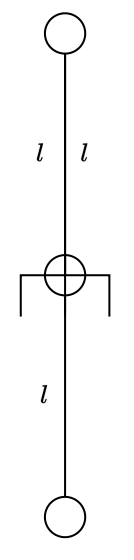
\includegraphics[width=0.25\linewidth]{ConfigurazioneQ2.png}
\end{minipage}
\hfill
\begin{minipage}[c]{0.65\textwidth}
    Sostituendo questi valori nel Jacobiano, otteniamo una matrice dall'aspetto molto differente:
    \[
        \bm{J}_r(\bm{q}_2) =
        \begin{bmatrix}
            0 & 0 & 0 \\
            3 & 2 & 1
        \end{bmatrix}
    \]
\end{minipage}

L'analisi di questa matrice rivela immediatamente una drastica perdita di mobilità.

\subparagraph{Rango e Spazio Immagine}
A colpo d'occhio, notiamo che la prima riga della matrice è nulla. Questo implica che la componente $\dot{x}$ della velocità dell'end-effector sarà sempre zero, indipendentemente dalle velocità dei giunti. Inoltre, tutte le colonne sono chiaramente multipli del vettore $\begin{bmatrix}0 \\ 1\end{bmatrix}$, e quindi sono linearmente dipendenti. Il rango della matrice è quindi $\rho(\bm{J}_r(\bm{q}_2)) = 1$.

Poiché il rango è strettamente minore della dimensione dello spazio del compito ($\rho < m$), la configurazione \textbf{è singolare}. Lo spazio delle velocità possibili non è più un piano, ma degenera in una linea:
\[
    R(\bm{J}_r(\bm{q}_2)) = \mathrm{span}\left\{ \begin{bmatrix} 0 \\ 1 \end{bmatrix} \right\}
\]
Il robot ha perso un grado di libertà operativo. In questa configurazione, l'end-effector può muoversi istantaneamente solo lungo l'asse $y$ (direzione verticale). È diventato \textbf{impossibile} generare una velocità lungo la direzione radiale (l'asse $x$), che è proprio la direzione di allineamento dei bracci. Questo tipo di singolarità, che si verifica ai confini dello spazio di lavoro, è comunemente detta \textbf{singolarità di bordo}.

\subparagraph{Nucleo}
Con la perdita di mobilità esterna, il robot guadagna mobilità interna. La dimensione dello spazio nullo aumenta: $\dim(N(\bm{J}_r(\bm{q}_2))) = n - \rho = 3 - 1 = 2$. Questo significa che ora esistono due direzioni di automovimento linearmente indipendenti; ci sono più modi per muovere i giunti mantenendo l'end-effector fermo.

\paragraph{Conclusioni Analisi}
\mbox{}\\ % Forza l'inizio di una nuova linea
Questa analisi su due semplici configurazioni dimostra il potente ruolo diagnostico del Jacobiano. L'algebra matriciale ci permette non solo di etichettare una posa come "singolare" o "non singolare", ma ci offre una profonda comprensione geometrica e quantitativa della mobilità del manipolatore in ogni istante. Lo \textbf{spazio immagine} definisce l'universo delle velocità raggiungibili dall'end-effector, mentre il \textbf{nucleo} caratterizza la ricchezza dei moti interni (automovimenti) che non influenzano il compito, una caratteristica intrinseca dei sistemi ridondanti.

\newpage

\subsection{Cinematica Differenziale Inversa}
Il problema della cinematica inversa, ovvero la determinazione delle variabili di giunto \(\bm{q}\) a partire da una data posa dell'end-effector, è intrinsecamente complesso a causa della non linearità delle sue equazioni. Un approccio alternativo e più gestibile consiste nell'operare a livello di velocità attraverso la cinematica differenziale. La relazione fondamentale, \(\bm{v}_e = \bm{J}(\bm{q})\dot{\bm{q}}\), stabilisce una trasformazione \textbf{lineare} tra il vettore delle velocità dei giunti \(\dot{\bm{q}}\) e quello delle velocità dell'end-effector \(\bm{v}_e\) per una configurazione \(\bm{q}\) nota. L'obiettivo diventa quindi calcolare le velocità dei giunti \(\dot{\bm{q}}(t)\) necessarie per tracciare una desiderata traiettoria di velocità dell'end-effector \(\bm{v}_e(t)\).

Nel caso ideale di un manipolatore \textbf{non-ridondante} (\(n=m\)), dove il numero di giunti \(n\) eguaglia la dimensione \(m\) dello spazio del compito, la matrice Jacobiana \(\bm{J}(\bm{q})\) è quadrata. Se il robot opera lontano da configurazioni singolari, la Jacobiana ha rango pieno ed è \textbf{invertibile}. In queste circostanze, la soluzione è ottenuta tramite una semplice inversione algebrica:
\[
    \dot{\bm{q}}(t) = \bm{J}^{-1}(\bm{q}(t)) \cdot \bm{v}_e(t)
\]
La traiettoria delle posizioni \(\bm{q}(t)\) può essere poi ricostruita per integrazione numerica. Ad esempio, con il \textbf{metodo di Eulero (In Avanti)}, la posizione al passo successivo è approssimata come \(\bm{q}(t_{k+1}) \approx \bm{q}(t_k) + \dot{\bm{q}}(t_k) \cdot \Delta t\), dove \(\Delta t\) è l'intervallo di tempo.

Tuttavia, l'applicabilità di questo approccio diretto è  limitata, poiché fallisce in due situazioni comuni e critiche. La prima riguarda i \textbf{manipolatori ridondanti} (\(n > m\)), dove la Jacobiana è una matrice rettangolare \(m \times n\) non invertibile, il che implica l'esistenza di infinite soluzioni \(\dot{\bm{q}}\) per la stessa \(\bm{v}_e\). La seconda si verifica in corrispondenza di \textbf{singolarità cinematiche} (\(\rho(\bm{J}) < m\)), configurazioni in cui la Jacobiana perde di rango (\(\det(\bm{J}) = 0\)) e la sua inversa non esiste, portando a velocità di giunto teoricamente infinite.

Per superare questi limiti e formulare una soluzione generale, si ricorre alla \textbf{\textit{Pseudo-Inversa di Moore-Penrose}}, denotata con \(\bm{J}^{\dagger}\). Questo strumento estende il concetto di inversa a matrici di qualsiasi dimensione, anche singolari, garantendo una soluzione al sistema lineare \(\bm{J}\dot{\bm{q}} = \bm{v}_e\) con importanti proprietà di ottimalità. La pseudo-inversa \(\bm{J}^\dagger\) è l'unica matrice che soddisfa le quattro condizioni di Penrose e la sua forma analitica dipende dalle proprietà di \(\bm{J}\):
\begin{itemize}
    \item Se \(\bm{J}\) è quadrata e non singolare, la pseudo-inversa coincide con l'inversa classica: \(\bm{J}^\dagger = \bm{J}^{-1}\).
    \item Per un robot ridondante (\(n > m\)) con Jacobiana a rango pieno (\(\rho(\bm{J}) = m\)), si utilizza la \textbf{pseudo-inversa destra}: \( \bm{J}^\dagger = \bm{J}^T(\bm{J}\bm{J}^T)^{-1} \).
    \item Per un robot sottodeterminato (\(m > n\)) con Jacobiana a rango pieno (\(\rho(\bm{J}) = n\)), si impiega la \textbf{pseudo-inversa sinistra}: \( \bm{J}^\dagger = (\bm{J}^T\bm{J})^{-1}\bm{J}^T \).
\end{itemize}
Quando un robot è ridondante, il sistema \(\bm{J}\dot{\bm{q}} = \bm{v}_e\) ammette infinite soluzioni. La pseudo-inversa permette di caratterizzarle tutte scomponendo la soluzione generale in due componenti ortogonali:
% \[
%     \dot{\bm{q}} = \dot{\bm{q}}_p + \dot{\bm{q}}_h
% \]
% Dove:
\begin{enumerate}
    \item La \textbf{Soluzione Particolare} \(\dot{\bm{q}}_p\). Questa è la componente che esegue il compito primario, cioè genera la velocità \(\bm{v}_e\) richiesta per l'end-effector. Utilizzando la pseudo-inversa, si ottiene la soluzione che tra tutte quelle infinite possibili è quella a \textbf{norma minima}:
    \[
        \dot{\bm{q}}_p = \bm{J}^{\dagger}\bm{v}_e
    \]
    Minimizzare la norma euclidea \(\|\dot{\bm{q}}\|\) significa trovare la soluzione che richiede le velocità istantanee dei giunti più basse possibili per compiere il movimento.

    \item La \textbf{Soluzione Omogenea} \(\dot{\bm{q}}_h\). Questa è la componente che sfrutta i gradi di libertà in eccesso, cioè genera un \textbf{automovimento} che riconfigura internamente il robot senza produrre alcun movimento dell'end-effector. Questa componente appartiene al \textbf{nucleo} della Jacobiana. I vettori in questo spazio hanno la proprietà che, se moltiplicati per \(\bm{J}\), danno come risultato il vettore nullo (\(\bm{J}\dot{\bm{q}}_h = \bm{0}\)). Sapendo che, qualsiasi vettore del nucleo può essere generato proiettando un vettore arbitrario \(\bm{y}_0\) di dimensione \(n\) sul nucleo, utilizzando la matrice (\(\bm{I} - \bm{J}^{\dagger}\bm{J}\)), possiamo esprimere la soluzione omogenea come:
    \[
        \dot{\bm{q}}_h = (\bm{I} - \bm{J}^{\dagger}\bm{J})\bm{y}_0
    \]
\end{enumerate}
Unendo queste due componenti, si ottiene la \textbf{Soluzione Generale Completa}:
\[
    \dot{\bm{q}} = \underbrace{\bm{J}^{\dagger}\bm{v}_e}_{\text{Compito Primario}} + \underbrace{(\bm{I} - \bm{J}^{\dagger}\bm{J})\bm{y}_0}_{\text{Compito Secondario (Automovimento)}}
\]
Il primo termine assicura che il robot esegua il suo compito primario, mentre il secondo termine permette di controllare il manipolatore per sfruttare i gradi di libertà in eccesso. Scegliendo opportunamente \(\bm{y}_0\), possiamo imporre compiti secondari come evitare ostacoli o mantenersi lontani dai limiti meccanici dei giunti.

\subsubsection{Gestione delle Singolarità: La Pseudo-Inversa Smorzata}
Quando un robot si avvicina a una configurazione singolare, il calcolo della pseudo-inversa standard diventa instabile e tende a divergere, generando velocità dei giunti eccessivamente elevate e fisicamente irrealizzabili. Per ovviare a questo problema critico, si utilizza un approccio di regolarizzazione noto come \textbf{Damped Least-Squares (DLS)} o pseudo-inversa smorzata.

L'idea fondamentale è quella di modificare l'obiettivo: invece di cercare una soluzione esatta a ogni costo, si cerca un compromesso ottimale tra l'accuratezza nell'esecuzione del compito e la norma delle velocità dei giunti. Questo si traduce nella minimizzazione di una nuova funzione di costo:
\[
    \min_{\dot{\bm{q}}} \left( \| \bm{J}\dot{\bm{q}} - \bm{v}_e \|^2 + k^2 \|\dot{\bm{q}}\|^2 \right)
\]
Il termine \(k \ge 0\) è un \textbf{fattore di smorzamento} (damping factor) che regola questo compromesso:
\begin{itemize}
    \item Se \(k=0\), si dà priorità assoluta all'accuratezza, ritrovando la soluzione standard.
    \item Se \(k>0\), si penalizzano le velocità dei giunti troppo elevate, accettando un piccolo e controllato errore di tracking sull'end-effector (\(\bm{J}\dot{\bm{q}} \neq \bm{v}_e\)).
\end{itemize}
La soluzione che minimizza questa funzione di costo è data dalla \textbf{pseudo-inversa smorzata}, denotata con \(\bm{J}^*\):
\[
    \dot{\bm{q}} = \bm{J}^* \bm{v}_e \quad \text{con} \quad \bm{J}^* = \bm{J}^T (\bm{J}\bm{J}^T + k^2\bm{I})^{-1}
\]
La forza di questo approccio risiede nell'aggiunta del termine \(k^2\bm{I}\). Questo termine "rinforza" la diagonale della matrice \(\bm{J}\bm{J}^T\), garantendo che la nuova matrice \((\bm{J}\bm{J}^T + k^2\bm{I})\) sia \textbf{sempre invertibile} e ben condizionata, anche quando \(\bm{J}\) è singolare.

Questo metodo assicura che la soluzione per \(\dot{\bm{q}}\) rimanga sempre stabile e finita, permettendo al robot di attraversare le singolarità in modo controllato. Il prezzo da pagare è un momentaneo sacrificio della precisione del tracking, una scelta pragmatica per mantenere la stabilità e la fattibilità fisica del movimento.

Per completezza, si richiamano le quattro proprietà fondamentali della \textbf{pseudo-inversa standard di Moore-Penrose}, \(\bm{J}^\dagger\), che la definiscono in modo univoco:
\begin{itemize}
    \item \(\bm{J}\bm{J}^\dagger\bm{J} = \bm{J}\)
    \item \(\bm{J}^\dagger\bm{J}\bm{J}^\dagger = \bm{J}^\dagger\)
    \item \((\bm{J}\bm{J}^\dagger)^T = \bm{J}\bm{J}^\dagger\) (la proiezione sull'immagine di \(\bm{J}\) è Hermitiana)
    \item \((\bm{J}^\dagger\bm{J})^T = \bm{J}^\dagger\bm{J}\) (la proiezione sul dominio di \(\bm{J}^T\) è Hermitiana)
\end{itemize}
Queste proprietà garantiscono che \(\bm{J}^\dagger\) agisca come la migliore approssimazione possibile di un'inversa nel senso dei minimi quadrati.

\newpage
\subsection{Esempio: Comportamento Singolarità Robot RR Planare}
\noindent
\begin{minipage}[c]{0.48\textwidth}
    \begin{tikzpicture}[scale=2]
        % Assi con frecce
        \draw[->] (0,0) -- (4,0) node[right] {$x$}; % Asse X
        \draw[->] (0,0) -- (0,3) node[above] {$y$}; % Asse Y

        % --- Definizione dei Punti Chiave tramite Coordinate ---
        % I punti sono calcolati per un angolo di 30 gradi
        \coordinate (Base) at (0,0);
        \coordinate (Joint2) at ({cos(30)}, {sin(30)});
        \coordinate (EndEffector) at ({2*cos(30)}, {2*sin(30)});

        % --- Disegno del Robot ---
        % Bracci del robot
        % $l_1$
        \draw[line width=1.5pt] (Base) -- (Joint2) node[midway, above] {};

        % $l_2$
        \draw[line width=1.5pt] (Joint2) -- (EndEffector) node[midway, below left, inner sep=2pt] {};

        % Giunti del robot
        \draw[fill=white, draw=black, line width=0.5pt] (Base) circle (0.1);
        \draw[fill=white, draw=black, line width=0.5pt] (Joint2) circle (0.1);
        \draw[fill=white, draw=black, line width=0.5pt] (EndEffector) circle (0.1);


        % --- Disegno della Pinza (End-Effector) ---
        \begin{scope}[shift={(EndEffector)}, rotate={30-90}, line width=1.5pt, draw=black]
            % Geometria della pinza disegnata localmente
            \draw (-0.2, 0) -- (0.2, 0);
            \draw (-0.2, 0) -- (-0.2, 0.2);
            \draw (0.2, 0) -- (0.2, 0.2);
        \end{scope}

        % Spazio Immagine R(J) - Tangenziale al movimento
        % $R(\bm{J})$
        \draw[thick, blue, dashed] ($(EndEffector) + (120:1)$) -- ($(EndEffector) + (120:-1)$) node[pos=0.15, anchor=south east] {};

        % Spazio Nullo N(J^T) - Radiale, non raggiungibile
        % $N(\bm{J}^T)$
        \draw[thick, red, dashed] ($(EndEffector) + (30:1.5)$) -- ($(EndEffector) + (30:0)$) node[pos=0.15, anchor=south west] {};

        % Etichette
        \node[text=red] at (3.25,1.5) {$N(J)$};
        \node[text=blue] at (1.5,2) {$R(J)$};
        \node at (1.25,1) {$l_{2}$};
        \node at (0.25,0.5) {$l_{1}$};
    \end{tikzpicture}
\end{minipage}
\hfill
\begin{minipage}[c]{0.48\textwidth}
Per comprendere a fondo le implicazioni di una configurazione singolare, consideriamo un semplice robot planare a due bracci (RR), ciascuno di lunghezza unitaria ($l_1 = l_2 = 1$). Analizziamo il caso di una \textbf{singolarità di bordo}, una delle configurazioni singolari più intuitive, che si verifica quando il secondo giunto ha un angolo nullo ($q_2 = 0$). In questa situazione, i due bracci sono completamente estesi e allineati, formando un'unica linea retta.

Il legame tra le velocità dei giunti ($\dot{\bm{q}}$) e la velocità dell'organo terminale ($\bm{v}_e$) è descritto dalla matrice Jacobiana. Quando $q_2 = 0$, e utilizzando le notazioni $s_1 = \sin(q_1)$ e $c_1 = \cos(q_1)$, lo Jacobiano assume la seguente forma:
\end{minipage}
\[
    \bm{J}(q_1, 0) = \begin{bmatrix} -l_1s_1 - l_2s_1 & -l_2s_1 \\ l_1c_1 + l_2c_1 & l_2c_1 \end{bmatrix} = \begin{bmatrix} -2s_1 & -s_1 \\ 2c_1 & c_1 \end{bmatrix}
\]
Un'analisi di questa matrice rivela immediatamente la natura della singolarità:
\begin{itemize}
    \item \textbf{Dal Punto Di Vista Algebrico} le due colonne della matrice sono linearmente dipendenti; la prima colonna è semplicemente il doppio della seconda. Questo significa che il rango della matrice è 1 ($\rho(\bm{J})=1$), un valore inferiore alla dimensione dello spazio di lavoro ($m=2$). Matematicamente, questo è il segnale inequivocabile di una singolarità.

    \item \textbf{Dal Punto Di Vista Fisico} il vettore $\begin{bmatrix}-s_1 \\ c_1\end{bmatrix}$ rappresenta una direzione di velocità perpendicolare all'asse del braccio esteso. Poiché entrambe le colonne della Jacobiana sono multiple di questo vettore, entrambi i giunti possono generare velocità dell'end-effector solo lungo questa direzione. Di conseguenza, il robot ha perso una delle sue capacità di movimento: può muoversi solo in direzione \textbf{tangenziale} (lungo la circonferenza di raggio massimo), ma non può più muoversi in direzione \textbf{radiale} (cioè allungarsi o accorciarsi).
\end{itemize}

Per capire cosa succede se si tenta di imporre una velocità che il robot non può fisicamente eseguire in questa configurazione, si utilizza la soluzione standard della cinematica inversa differenziale, basata sulla pseudo-inversa di Moore-Penrose ($\bm{J}^\dagger$).

Consideriamo la configurazione specifica in cui il braccio è orientato a 30 gradi, ovvero $q_1 = \pi/6$. Lo Jacobiano numerico diventa:
\[
    \bm{J} = \begin{bmatrix} -2\sin(\pi/6) & -\sin(\pi/6) \\ 2\cos(\pi/6) & \cos(\pi/6) \end{bmatrix} = \begin{bmatrix} -1 & -1/2 \\ \sqrt{3} & \sqrt{3}/2 \end{bmatrix}
\]
Imponendo una velocità desiderata puramente orizzontale, $\bm{v}_e = [-1/2, 0]^T$, poiché il braccio del robot è inclinato, per muoversi orizzontalmente l'end-effector dovrebbe necessariamente anche ritrarsi, ovvero avere una componente di velocità radiale. Ma abbiamo appena stabilito che questo è impossibile. La velocità $\bm{v}_e$ non appartiene allo spazio delle velocità raggiungibili, noto come immagine dello Jacobiano ($R(\bm{J})$).

La velocità che l'end-effector effettivamente produce è data da $\bm{v}_{actual} = \bm{J}\dot{\bm{q}} = \bm{J}\bm{J}^\dagger \bm{v}_e$. L'operatore $\bm{J}\bm{J}^\dagger$ agisce come un \textbf{proiettore ortogonale}. In termini semplici, "prende" il vettore della velocità desiderata $\bm{v}_e$ e lo proietta sullo spazio delle velocità che il robot può effettivamente generare ($R(\bm{J})$). Il risultato è il vettore $\bm{v}_{actual}$, che è il vettore raggiungibile più vicino a quello desiderato. È come se trovasse "l'ombra" della velocità richiesta sul piano dei movimenti possibili.
\newpage
Svolgendo i calcoli si ottiene:
\[
    \bm{v}_{actual} = \bm{J}\bm{J}^\dagger\bm{v}_e =
    \begin{bmatrix}
        -1/8 \\
        \sqrt{3}/8
    \end{bmatrix}
\]
Questo risultato è molto diverso dalla velocità desiderata $\bm{v}_e$ ed è fondamentale per capire il comportamento del controllo in singolarità:
\begin{itemize}
    \item L'approccio basato su pseudo-inversa \textbf{non riesce a realizzare una velocità desiderata} se questa ha una componente impossibile.
    \item Tuttavia, non fallisce completamente. Fornisce la \textbf{migliore approssimazione possibile} secondo la norma Euclidea, proiettando il comando sullo spazio dei movimenti realizzabili. L'errore di inseguimento ($\bm{v}_e - \bm{v}_{actual}$) risulta essere ortogonale a tale spazio.
\end{itemize}

Se la velocità desiderata $\bm{v}_e$ fosse stata già realizzabile (ad esempio, una velocità puramente tangenziale), la soluzione sarebbe stata esatta, con $\bm{v}_{actual} = \bm{v}_e$.

\newpage

\section{Ellissoidi di Manipolabilità}
Gli \textbf{ellissoidi di manipolabilità} sono lo strumento geometrico che ci permette di capire "quanto bene" il robot possa muoversi in una certa direzione. Essi rappresentano una mappa delle prestazioni cinematiche del robot in una specifica configurazione $\bm{q}$.

L'utilità di questi indici si manifesta principalmente in due ambiti:
\begin{itemize}
    \item \textbf{Fase Di Progettazione:} Poichè ci permettono di confrontare diverse architetture cinematiche o lunghezze dei link per massimizzare l'area di lavoro utile.
    \item \textbf{Fase Di Pianificazione:} Poichè ci aiutano a selezionare traiettorie che mantengano il robot lontano da configurazioni singolari.
\end{itemize}

\subsection{Ellissoide Di Manipolabilità In Velocità}
L'ellissoide di manipolabilità in velocità permette di capire quale \emph{quale insieme di velocità cartesiane è in grado di generare l'end-effector date le velocità disponibili per i giunti}. \\
Poiché lo Jacobiano è una funzione di $\bm{q}$, la capacità di movimento varia al variare della posa del robot, quindi vogliamo capire se il manipolatore è ugualmente veloce in tutte le direzioni (isotropo) o se privilegia certi assi di movimento a discapito di altri.\\
L'insieme di tutti i vettori di velocità di giunto $\dot{\bm{q}}$ che hanno norma unitaria, rappresenta una condizione in cui la somma dei quadrati delle velocità dei giunti è limitata a un valore costante normalizzato a 1.\\
Nello spazio dei giunti (di dimensione \(n\), questa condizione descrive una \textbf{ipersfera} unitaria definita dall'equazione:
\[
    \|\dot{\bm{q}}\|^2 = \dot{\bm{q}}^T\dot{\bm{q}} = 1
\]
L'obiettivo è quello di mappare questa sfera nello spazio operativo che ha dimensione $m$ dimensioni. Quindi, per capire come la sfera si trasforma, si deve esprimere l'equazione della sfera in termini di $\bm{v}_e$ e questo richiede l'uso della cinematica differenziale inversa.

Generalmente (a causa dei robot ridondanti dove $n > m$), la matrice $\bm{J}$ non è quadrata e quindi non è direttamente invertibile. Esistono quindi infinite soluzioni per $\dot{\bm{q}}$ e tra queste quella che minimizza la norma delle velocità dei giunti è data dalla \textbf{pseudo-inversa destra} di Moore-Penrose:
\[
    \dot{\bm{q}} = \bm{J}^\dagger \bm{v}_e \qquad \qquad \qquad \text{con } \bm{J}^\dagger = \bm{J}^T (\bm{J}\bm{J}^T)^{-1}
\]
Sostituendo l'espressione di $\dot{\bm{q}}$ all'interno dell'equazione della sfera unitaria si ottiene:
\[
    (\bm{J}^\dagger \bm{v}_e)^T (\bm{J}^\dagger \bm{v}_e) = 1 \quad\underbrace{\quad \longrightarrow \quad}_{(\bm{A}\bm{B})^T = \bm{B}^T\bm{A}^T} \quad \bm{v}_e^T (\bm{J}^\dagger)^T \bm{J}^\dagger \bm{v}_e = 1
\]
Sostituendo la definizione esplicita di $\bm{J}^\dagger$:
\[
    \bm{v}_e^T \left[ \bm{J}^T (\bm{J}\bm{J}^T)^{-1} \right]^{T} \; \left[ \bm{J}^T (\bm{J}\bm{J}^T)^{-1} \right] \bm{v}_e = 1 \quad\underbrace{\quad \longrightarrow \quad}_{\bm{J}\bm{J}^T \text{Simmetrica}} \quad \bm{v}_e^T \left[ (\bm{J}\bm{J}^T)^{-1}\bm{J} \right] \left[ \bm{J}^T (\bm{J}\bm{J}^T)^{-1} \right] \bm{v}_e = 1
\]

\[
    \bm{v}_e^T (\bm{J}\bm{J}^T)^{-1} \underbrace{\bm{J} \bm{J}^T (\bm{J}\bm{J}^T)^{-1}}_{= I} \; \bm{v}_e = 1 \qquad \longrightarrow \qquad \bm{v}_e^T (\bm{J}\bm{J}^T)^{-1} \bm{v}_e = 1
\]
Quindi, l'equazione finale che descrive il luogo dei punti nello spazio delle velocità cartesiane è:
\[
    \bm{v}_e^T \left( \bm{J}(\bm{q})\bm{J}(\bm{q})^T \right)^{-1} \bm{v}_e = 1
\]
Questa è l'equazione di un \textbf{ellissoide} centrato nell'origine. La matrice $\bm{J}\bm{J}^T$ è il nucleo di questa rappresentazione ed è spesso chiamata \emph{matrice di manipolabilità}.

\subsubsection{Interpretazione Geometrica e Valori Singolari}
La forma e l'orientamento dell'ellissoide di manipolabilità sono determinati dalle proprietà della matrice \(\mathbf{A} = \mathbf{J}\mathbf{J}^T\). Essendo simmetrica e definita positiva (lontano dalle singolarità), la sua struttura può essere studiata tramite la Single Value Decomposition (SVD).

Quindi, possiamo scrivere \(\mathbf{J} \) come \(\mathbf{U}\,\mathbf{\Sigma}\,\mathbf{V}^T\), dove gli elementi sulla diagonale  di \(\mathbf{\Sigma}\) sono i valori singolari \(\sigma_i \ge 0\). Gli autovalori della matrice \(\mathbf{A} = \mathbf{J}\mathbf{J}^T\) coincidono con i quadrati dei valori singolari, quindi \(\lambda_i = \sigma_i^2\)

Dall'analisi degli autovalori e autovettori derivano le caratteristiche fisiche dell'ellissoide:

\begin{itemize}
    \item \textbf{Assi Principali:} La direzione degli assi dell'ellissoide è data dagli autovettori della matrice $\bm{J}\bm{J}^T$ che corrispondono alle colonne della matrice $\bm{U}$. Questi vettori indicano le direzioni nello spazio cartesiano lungo le quali avviene il movimento.

    \item \textbf{Lunghezza Dei Semiassi:} La lunghezza di ciascun semiasse è data dalla radice quadrata dell'autovalore corrispondente, ovvero $\sqrt{\lambda_i} = \sigma_i$.
    \begin{itemize}
        \item Un valore singolare $\sigma_i$ elevato implica che, in quella direzione (autovettore corrispondente), una piccola velocità ai giunti viene amplificata in una grande velocità cartesiana. Si dice che il robot ha una buona \emph{trasmissione cinematica} in quella direzione.
        \item Un valore singolare $\sigma_i$ basso implica che il robot fa fatica a generare velocità in quella direzione.
    \end{itemize}
\end{itemize}

\paragraph{Analisi Delle Configurazioni.}
Possiamo distinguere tre casi fondamentali osservando la forma dell'ellissoide:

\begin{minipage}{0.66\textwidth}
    \begin{enumerate}[left=0pt]
        \item \textbf{Configurazione Isotropa:} Se $\sigma_{max} = \sigma_{min}$ (tutti i valori singolari sono uguali), l'ellissoide diventa una \textbf{sfera}. In questo caso, il robot ha la stessa capacità di velocità in tutte le direzioni. Questa è la condizione ideale per la manipolabilità.

        \item \textbf{Configurazione Generica:} Solitamente l'ellissoide è allungato. La direzione dell'asse maggiore (associato a $\sigma_{max}$) indica la direzione di massima mobilità. La direzione dell'asse minore (associato a $\sigma_{min}$) è quella in cui il robot è più lento o meno agile.

        \item \textbf{Configurazione Singolare:} Se il robot raggiunge una singolarità cinematica, il Jacobiano perde rango. Questo significa che almeno uno dei valori singolari $\sigma_{min}$ diventa nullo. Geometricamente, l'ellissoide si "schiaccia" completamente lungo quella direzione, degenerando in un ellissoide di dimensione inferiore (un disco o un segmento nello spazio 3D). In quella direzione, la velocità realizzabile è nulla, indipendentemente dallo sforzo ai giunti.
    \end{enumerate}
\end{minipage}
\hfill
\begin{minipage}{0.33\textwidth}
    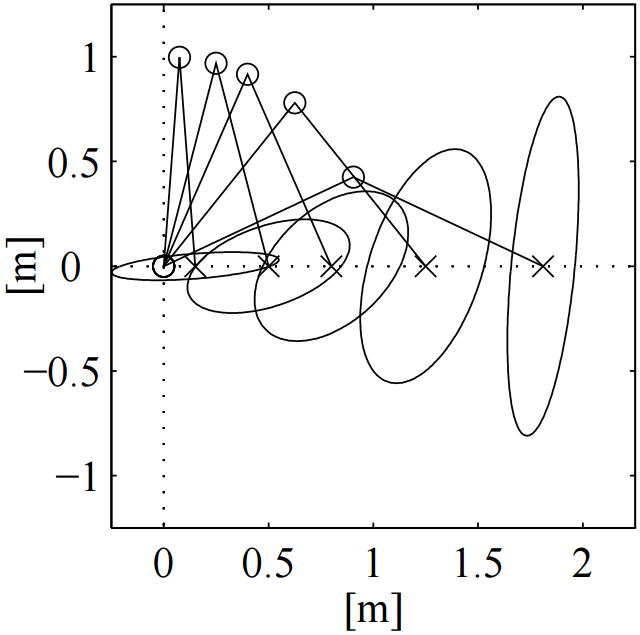
\includegraphics[width=1\textwidth]{Figura_3_23.png}
\end{minipage}

\newpage

%%%%%%%%%%%%%%%%%%%%%%%%%%%%%%%%%%%%%%%%%%%%%%%%%%%%%%%%%%%%%%%%%%%%%
\subsubsection{Indici Quantitativi di Manipolabilità}
Per permettere agli algoritmi di valutare numericamente una configurazione e di confrontarne diverse istante per istante è necessario condensare le informazioni della matrice $\bm{J}\bm{J}^T$ in valori scalari, detti \textit{indici di prestazione}.

\paragraph{Misura di Manipolabilità (Indice di Volume)}
L'indice più classico è la \textbf{misura di manipolabilità} $w(\bm{q})$. Geometricamente, questo scalare è proporzionale al \textbf{volume} dell'ellissoide di velocità. È definito come:
\[
    w(\bm{q}) = \sqrt{\det\left(\bm{J}(\bm{q})\bm{J}(\bm{q})^T\right)}
\]
Sfruttando le proprietà dell'algebra lineare, sappiamo che il determinante di una matrice è pari al prodotto dei suoi autovalori. Poiché gli autovalori di $\bm{J}\bm{J}^T$ sono i quadrati dei valori singolari $\sigma_i$ del Jacobiano, possiamo riscrivere l'indice come:
\[
    w(\bm{q}) = \sigma_1 \cdot \sigma_2 \cdot \dots \cdot \sigma_m
\]
Per un manipolatore non ridondante (dove $n=m$ e $\bm{J}$ è quadrata), questa espressione si semplifica ulteriormente in $w(\bm{q}) = |\det(\bm{J})|$.

\begin{itemize}
    \item Un valore elevato di $w$ indica che l'ellissoide ha un grande volume, suggerendo che il robot si trova in una configurazione "ben condizionata" dove può generare velocità con facilità.
    \item Se il robot raggiunge una singolarità, il valore singolare minimo $\sigma_{min}$ diventa nullo. Di conseguenza, il prodotto dei valori singolari si annulla: $w(\bm{q}) = 0$. Questo rende $w$ un ottimo indicatore per rilevare l'imminenza di una singolarità (il valore decresce rapidamente avvicinandosi ad essa).
\end{itemize}

Tuttavia, la misura di manipolabilità presenta due criticità:
\begin{enumerate}
    \item \textit{Dipendenza Dalla Scala:} L'indice non è adimensionale. Dipende dalle unità di misura e dalle dimensioni fisiche dei link. Un robot gigante avrà un $w$ molto più grande di un robot chirurgico, anche se la loro destrezza cinematica relativa fosse identica.
    \item \textit{Cecità Alla Forma:} Essendo un prodotto, $w$ non distingue tra un ellissoide sferico (buono) e uno molto schiacciato ma allungato (pessimo). Un ellissoide molto schiacciato può avere lo stesso volume di una sfera piccola, ma rappresenta una condizione vicina alla singolarità in certe direzioni.
\end{enumerate}

\paragraph{Numero di Condizionamento (Indice di Isotropia)}
Per ovviare ai problemi di scala e forma, si utilizza il \textbf{numero di condizionamento} della matrice Jacobiana, indicato con $\kappa(\bm{J})$. Esso è un indice adimensionale definito come il rapporto tra il massimo e il minimo valore singolare:
\[
    \kappa(\bm{J}) = \frac{\sigma_{\text{max}}}{\sigma_{\text{min}}} \quad \in [1, \infty)
\]
Geometricamente, questo valore rappresenta l'\textbf{eccentricità} dell'ellissoide, ovvero il rapporto tra la lunghezza dell'asse maggiore e quella dell'asse minore.
\begin{itemize}
    \item \textbf{Isotropia ($\kappa = 1$):} Si verifica quando $\sigma_{\text{max}} = \sigma_{\text{min}}$. L'ellissoide è una sfera perfetta. Il robot possiede la stessa capacità di movimento in tutte le direzioni. Questa è la configurazione ideale per la controllabilità uniforme.
    \item \textbf{Singolarità ($\kappa \to \infty$):} Quando ci si avvicina a una singolarità, $\sigma_{\text{min}}$ tende a zero, facendo esplodere il valore di $\kappa$. L'ellissoide diventa infinitamente schiacciato.
\end{itemize}
In sintesi, mentre $w$ misura "quanto" movimento globale si può generare, $\kappa$ misura l'\textbf{uniformità} di tale movimento. Nella progettazione di robot, si cerca spesso di mantenere $\kappa$ il più vicino possibile a 1 in tutto lo spazio di lavoro.
\newpage
\subsubsection{Ellissoide di Manipolabilità in Forza}
Grazie alla dualità cineto-statica, si possono analizzare la capacità del robot di esercitare forze statiche sull'ambiente. Ricordiamo la relazione fondamentale della statica che lega le coppie ai giunti $\bm{\tau}$ alle forze cartesiane all'end-effector $\bm{f}$:
\[
    \bm{\tau} = \bm{J}^T(\bm{q}) \bm{f}
\]
Per costruire l'ellissoide di forza, si procede in modo analogo a quello di velocità. Immaginiamo di limitare le coppie dei giunti a una sfera unitaria (sforzo attuativo normalizzato):
\[
    \bm{\tau}^T\bm{\tau} \leq 1
\]
Sostituendo la relazione statica nell'equazione della sfera, si ottiene:
\[
    (\bm{J}^T\bm{f})^T (\bm{J}^T\bm{f}) = 1
\]
Sviluppando il prodotto trasposto ($\bm{A}\bm{B})^T = \bm{B}^T\bm{A}^T$, arriviamo all'equazione quadratica:
\begin{equation}
    \bm{f}^T \left( \bm{J}(\bm{q})\bm{J}(\bm{q})^T \right) \bm{f} = 1
\end{equation}
Questa equazione descrive l'\textbf{ellissoide di manipolabilità in forza}. Esso rappresenta le forze applicabili dall'end-effector dato uno sforzo unitario ai giunti.

\paragraph{Il Principio di Dualità Cineto-Statica.}
Confrontiamo le equazioni dei due ellissoidi per cogliere un aspetto fondamentale della meccanica robotica:
\begin{itemize}
    \item \textbf{Velocità:} $\bm{v}_e^T \left( \bm{J}\bm{J}^T \right)^{-1} \bm{v}_e = 1$
    \item \textbf{Forza:} $\quad \bm{f}^T \left( \bm{J}\bm{J}^T \right) \bm{f} = 1$
\end{itemize}
Notiamo che le matrici centrali delle forme quadratiche sono l'una l'inversa dell'altra.
Dalla teoria delle forme quadratiche $\bm{x}^T\bm{A}\bm{x}=1$, sappiamo che la lunghezza dei semiassi è data da $1/\sqrt{\lambda_i(\bm{A})}$.

Considerando la SVD, gli autovalori di $\bm{J}\bm{J}^T$ sono $\sigma_i^2$. Ne consegue che:
\begin{itemize}
    \item I semiassi dell'ellissoide di \textbf{velocità} hanno lunghezza $\sigma_i$.
    \item I semiassi dell'ellissoide di \textbf{forza} hanno lunghezza $1/\sigma_i$.
\end{itemize}
Questo risultato matematico formalizza il \textbf{Principio di Dualità}:
\begin{quote}
    \emph{Le direzioni in cui il robot ha la massima capacità di velocità (alto rapporto di trasmissione) sono esattamente quelle in cui ha la minima capacità di forza (basso vantaggio meccanico), e viceversa.}
\end{quote}

Questa dualità guida le strategie di pianificazione del compito:
\begin{itemize}
    \item Se il compito richiede \textbf{grandi velocità} (es. movimenti rapidi a vuoto), bisogna allineare la direzione del moto con l'asse maggiore dell'ellissoide di velocità ($\sigma_{max}$).
    \item Se il compito richiede l'applicazione di \textbf{grandi forze}, bisogna allineare la direzione della forza con l'asse maggiore dell'ellissoide di forza. Attenzione: questo corrisponde all'asse \textit{minore} dell'ellissoide di velocità ($\sigma_{min}$).
\end{itemize}
In pratica, un robot vicino a una singolarità ($\sigma_{min} \approx 0$) non può muoversi in quella direzione, ma paradossalmente è in grado di resistere a forze esterne enormi lungo quella stessa direzione senza affaticare i motori (si pensi a un braccio completamente disteso che regge un peso: lo sforzo è tutto sulla struttura meccanica, non sulla coppia dei giunti).


\newpage
\paragraph{Esempio Applicativo: Il Compito della Scrittura.}

Per comprendere concretamente l'utilità degli ellissoidi, analizziamo un compito comune ma cinematicamente complesso: la scrittura su una superficie piana. Affinché un manipolatore (o il braccio umano) possa scrivere in modo efficace, deve soddisfare contemporaneamente due requisiti fisici contrastanti lungo direzioni ortogonali:

\begin{enumerate}
    \item \textbf{Direzione Verticale (Controllo di Forza):}
    Lungo l'asse $z$, perpendicolare al foglio, non è richiesto un movimento veloce, bensì la capacità di mantenere una pressione costante della penna sulla carta. È necessario compensare le irregolarità della superficie e l'attrito senza che la penna si stacchi o buchi il foglio.
    In termini di manipolabilità, ciò richiede che il robot sia in una configurazione in cui il vantaggio meccanico è massimo lungo la verticale. Pertanto, l'\textbf{ellissoide di manipolabilità in forza} deve avere il suo \textbf{asse maggiore orientato verticalmente}. Grazie al principio di dualità, questo implica che la capacità di velocità in questa direzione sarà minima, il che è accettabile poiché non dobbiamo muoverci verticalmente.

    \item \textbf{Direzione Orizzontale (Controllo di Velocità):}
    Sul piano $xy$ del foglio, il compito richiede di tracciare lettere e curve in modo fluido e rapido. Qui la forza richiesta è minima (solo quella necessaria a vincere l'attrito laterale), ma è fondamentale l'agilità cinematica.
    Di conseguenza, l'\textbf{ellissoide di manipolabilità in velocità} deve avere i suoi \textbf{assi maggiori giacenti sul piano orizzontale}. Ciò garantisce che piccole velocità ai giunti si traducano in ampi movimenti della penna, facilitando la scrittura.
\end{enumerate}

La configurazione ottimale per la scrittura è dunque quella che allinea gli assi principali degli ellissoidi con le direzioni naturali del compito (il cosiddetto \emph{Task Frame}).

È qui che entra in gioco la \textbf{ridondanza cinematica} (tipica del braccio umano a 7 gradi di libertà o dei robot collaborativi): un manipolatore ridondante può modificare la propria configurazione interna (i movimenti nel "null space") senza spostare la punta della penna, ruotando di fatto gli ellissoidi nello spazio fino a farli coincidere con le direzioni desiderate di forza e velocità.

\vspace{0.5cm}

\noindent
\begin{minipage}[c]{0.38\textwidth}
    \centering
    \resizebox{0.9\linewidth}{!}{%
        \begin{tikzpicture}
            % Piano di scrittura
            \draw[thick] (-2.5,0) -- (2.5,0) node[below right] {\small Piano di scrittura};

            % Penna stilizzata
            \draw[line width=1.5pt, fill=gray!30] (0,0.05) -- (0.2, 0.6) -- (-0.2, 0.6) -- cycle;
            \draw[thick, gray] (0, 0.6) -- (0, 2.3); % Asta penna/mano
            \node at (0,0) {$\bullet$};

            % Ellissoide di Forza (ROSSO) - Verticale
            % Indica alta capacità di forza verso il basso (pressione)
            \draw[red, thick, dashed] (0,0.8) ellipse (0.4cm and 1.2cm);
            \node[red, font=\footnotesize] at (1.1, 1.5) {Forza ($\bm{f}$)};
            % \draw[->, red] (0.5, 1.5) -- (0.1, 1.0);

            % Ellissoide di Velocità (BLU) - Orizzontale
            % Indica alta capacità di movimento laterale (scrittura)
            \draw[blue, thick, dashed] (0,0.8) ellipse (1.6cm and 0.5cm);
            \node[blue, font=\footnotesize] at (2.0, 0.25) {Velocità ($\bm{v}$)};
            % \draw[->, blue] (1.8, 0.6) -- (1.2, 0.8);

            % Assi cartesiani di riferimento locale
            \draw[->, thin] (-2, 2) -- (-1.5, 2) node[right] {$x$};
            \draw[->, thin] (-2, 2) -- (-2, 2.5) node[above] {$z$};
        \end{tikzpicture}
    }
\end{minipage}
\hfill
\begin{minipage}[c]{0.58\textwidth}
    \textbf{Interpretazione Grafica:}
    La figura mostra la configurazione ideale per la scrittura.
    \begin{itemize}
        \item L'\textcolor{blue}{ellissoide di velocità (blu)} è allungato orizzontalmente, indicando che il robot è "agile" nel tracciare le lettere sul piano.
        \item L'\textcolor{red}{ellissoide di forza (rosso)} è allungato verticalmente, indicando che il robot può esercitare o controllare efficacemente la pressione verso il basso.
    \end{itemize}
    Si noti la relazione di dualità: dove l'ellissoide blu è largo, quello rosso è stretto, e viceversa.
\end{minipage}

\vspace{0.5cm}

In conclusione, gli ellissoidi di manipolabilità trascendono il concetto di semplice indice numerico. Essi costituiscono uno strumento concettuale indispensabile per verificare la \textbf{compatibilità} tra la struttura cinematica del robot e i requisiti fisici del compito assegnato, guidando sia la progettazione meccanica che le strategie di controllo.
\end{document}
